\documentclass[11pt]{article}
%% preamble.tex
%% this should be included with a command like
%% %% preamble.tex
%% this should be included with a command like
%% %% preamble.tex
%% this should be included with a command like
%% \input{p}

\usepackage{amsfonts}
\usepackage{amsthm}
\usepackage{latexsym}
\usepackage{amsmath}
%\usepackage{newalg}
\usepackage{amssymb}
\usepackage{latexsym}
\usepackage{subfigure}
\usepackage{graphicx}
\usepackage{wasysym}
\usepackage{booktabs}
\usepackage{hyperref}
\usepackage{mathtools}
\usepackage[makeroom]{cancel}
\usepackage{enumerate}
\usepackage{framed}
\usepackage{tikz}
\usepackage{mdframed}
\usepackage{algorithm}
\usepackage[noend]{algpseudocode}

% THEOREMS AND DEFINITIONS
\newcommand{\sk}{s}
\newtheorem{theorem}{Theorem}
\newtheorem{lesson}{Lesson}
\newtheorem{proposition}{Proposition}
\newtheorem{lemma}{Lemma}
\newtheorem{corollary}{Corollary}
\newtheorem{fact}{Fact}
\newtheorem*{claim}{Claim}
%\theoremstyle{definition}
\newtheorem{definition}{Definition}
\newtheorem{assumption}{Assumption}
\theoremstyle{remark}
\newtheorem{example}{Example}
\newtheorem*{remark}{Remark}

% DEFINITION command
%\newcounter{definitionCount}
%\setcounter{definitionCount}{0}
%\newcommand{\definition}[1]{
%\addtocounter{definitionCount}{1}
%\begin{mdframed}[backgroundcolor=gray!3,roundcorner=4pt]\textbf{ Definition \arabic{definitionCount}:} #1
%\end{mdframed}}

%==============================================================================
% Macros.
%==============================================================================
\newcommand{\new}[1]{{\em #1\/}}		% New term (set in italics).
\newcommand{\set}[1]{\{#1\}}			% Set (as in \set{1,2,3})
\newcommand{\setof}[2]{\{\,{#1}|~{#2}\,\}}	% Set (as in \setof{x}{x > 0})
\newcommand{\C}{\mathbb{C}}	                % Complex numbers.
\newcommand{\Q}{\textsf{Q}}                     % Robinson Arithmetic
\newcommand{\R}{\textsf{R}}                     % The system R
\newcommand{\PA}{\textsf{PA}}                     % Peano Arithmetic
\newcommand{\LA}{$\mathcal{LA}$}			% Language of Arithmetic
\newcommand{\compl}[1]{\overline{#1}}		% Complement of ...     
\newcommand{\subproblem}[1]{\vspace{4 mm}\noindent {\bf (#1)} \\} % Subproblem (a), (b), etc...
\newcommand{\elem}[1]{\noindent{\bf #1}}	    % Proof element (Claim:, Proof:, etc.)
\newcommand{\spacerule}{\vspace{4mm}\hrule\vspace{4mm}} % Add an hrule with some space
\newcommand{\dmod}[2]{\left[ #1\ \text{mod}\ #2\right]} % My mod rule
\newcommand{\tab}[1]{\hspace{.2\textwidth}\rlap{#1}}

\newcommand{\ra}[1]{\renewcommand{\arraystretch}{#1}} % booktabs table cmd for spacing

% Misc lines and other formatting
\newcommand{\encircle}[1]{\tikz[baseline=(char.base)]\node[anchor=south west, draw,rectangle, rounded corners, inner sep=2pt, minimum size=6mm, text height=2mm](char){#1} ;} % Circled text
\newcommand{\midline}{
\begin{center}
\noindent\rule{4cm}{0.4pt}
\end{center}}

% GODEL NUMBERS
\newbox\gnBoxA
\newdimen\gnCornerHgt
\setbox\gnBoxA=\hbox{$\ulcorner$}
\global\gnCornerHgt=\ht\gnBoxA
\newdimen\gnArgHgt
\def\Godelnum #1{%
\setbox\gnBoxA=\hbox{$#1$}%
\gnArgHgt=\ht\gnBoxA%
\ifnum     \gnArgHgt<\gnCornerHgt \gnArgHgt=0pt%
\else \advance \gnArgHgt by -\gnCornerHgt%
\fi \raise\gnArgHgt\hbox{$\ulcorner$} \box\gnBoxA %
\raise\gnArgHgt\hbox{$\urcorner$}}

\DeclarePairedDelimiter{\ceil}{\lceil}{\rceil}
\DeclareSymbolFont{AMSb}{U}{msb}{m}{n}
\DeclareMathSymbol{\F}{\mathalpha}{AMSb}{"46}
\DeclareMathSymbol{\N}{\mathalpha}{AMSb}{"4E}
\DeclareMathSymbol{\X}{\mathalpha}{AMSb}{"58}
\DeclareMathSymbol{\Zz}{\mathalpha}{AMSb}{"5A}
\DeclareMathOperator*{\argmin}{arg\,min}
\DeclareMathOperator*{\argmax}{arg\,max}
\newcommand{\Z}[1]{{\ensuremath{\Zz_{#1}} }}
\newcommand{\Zs}[1]{\ensuremath{\Zz^{\ast}_{#1}}}
\newcommand{\Zn}{\Z{n}}
\newcommand{\Zns}{\Zs{n}}
\newcommand{\Zstar}[1]{\Zs{#1}}
\newcommand{\Zp}{{\Z{p}}}
\newcommand{\Zps}{\Zs{p}}
\newcommand{\Zqs}{\Zs{q}}
\newcommand{\Zq}{{\Z{q}}}
%\newcommand{\QR}{\mathop{\mathrm{QR}}\nolimits}
\newcommand{\ord}[1]{\mathop{\mathrm{ord}}({#1})}
\newcommand{\QR}[1]{\ensuremath{\textit{QR}_{#1}}}
\newcommand{\becomes}{:=}
\newcommand{\rem}[1]{\ensuremath{\ \operatorname{rem} #1}}  
\newcommand{\U}{{\mathcal{U}}}
\newcommand{\floor}[1]{\ensuremath{\lfloor{#1}\rfloor}}
\newcommand{\de}[1]{\ensuremath{\Delta{#1}}}
\newcommand{\js}[2]{\left( \frac{#1}{#2} \right)}
\newcommand{\E}[1]{{\bf E} \left[ #1 \right]}
\newcommand{\PR}[1]{{\bf Pr} \left[ #1 \right]}

\renewcommand{\QR}{{\mbox{QR}}}
\newcommand{\QNR}{{\mbox{QNR}}}
\newcommand{\crt}{{\mbox{CRT}}}
\newcommand{\rsa}{{\mbox{RSA}}}
\newcommand{\rsamod}{{\mbox{RSA-modulus}}}


\newcommand{\greq}[1]{\stackrel{#1}{=}}
\newcommand{\hash}{\ensuremath{\mathcal{H}}}
\newcommand{\negl}{{\tt neg}}
\newcommand{\cindist}{\stackrel{c}{\approx}}
\newcommand{\A}{{\mathcal{A}}}
\newcommand{\B}{{\mathcal{B}}}

\newcommand{\gen}{\mathit{Gen}}
\newcommand{\keygen}{\mathit{KeyGen}}
\newcommand{\RSA}{\mathit{RSA}}
\newcommand{\pk}{\mathit{pk}}
\newcommand{\PK}{\mathit{PK}}
\newcommand{\SK}{\mathit{SK}}
\newcommand{\sign}{\mathit{Sign}}
\newcommand{\verify}{\mathit{Verify}}

% Bew command
\newcommand{\Bew}[1]{\textsc{Bew}(\Godelnum{#1})}


\setlength{\oddsidemargin}{.25in}
\setlength{\evensidemargin}{.25in}
\setlength{\textwidth}{6in}
\setlength{\topmargin}{-0.4in}
\setlength{\textheight}{8.5in}

\newcommand{\handout}[5]{
   \renewcommand{\thepage}{#1-\arabic{page}}
   \noindent
   \begin{center}
   \framebox{
      \vbox{
    \hbox to 5.78in { {\bf PHIL1885: Incompleteness} \hfill #2 }
       \vspace{4mm}
       \hbox to 5.78in { {\Large \hfill #5  \hfill} }
       \vspace{2mm}
       \hbox to 5.78in { {\it #3 \hfill #4} }
      }
   }
   \end{center}
   \vspace*{4mm}
}

% REMOVES ALL INDENTATION
%\setlength{\parindent}{0pt}

\usepackage{parskip}

\newcommand{\ho}[4]{\handout{#1}{#2}{Instructor:
#3}{}{Handout #1: #4}}

\newcommand{\lnotes}[3]{\handout{#1}{#2}{Instructor:
#3}{}{Lecture #1}}

\newcommand{\solution}[1]{#1}
%\homework{number}{out}{due}{instructor}
\newcommand{\homework}[4]{\handout{HW #1}{#2}{Instructor: #4}{Due: #3}{Homework #1}}

%================================================
% problemset macros
%================================================
% count problems
%\newcounter{solutioncount}
%\setcounter{solutioncount}{0}
\newcommand{\problem}[1]{%
%\addtocounter{solutioncount}{1}%
\section*{Problem #1:}}

% lets you make alphabetical lists (at first-level of enumeration)
\newenvironment
  {alphabetize}{\renewcommand{\theenumi}{\alph{enumi}}\begin{enumerate}}
  {\end{enumerate}\renewcommand{\theenumi}{\arabic{enumi}}}

\usepackage{amsfonts}
\usepackage{amsthm}
\usepackage{latexsym}
\usepackage{amsmath}
%\usepackage{newalg}
\usepackage{amssymb}
\usepackage{latexsym}
\usepackage{subfigure}
\usepackage{graphicx}
\usepackage{wasysym}
\usepackage{booktabs}
\usepackage{hyperref}
\usepackage{mathtools}
\usepackage[makeroom]{cancel}
\usepackage{enumerate}
\usepackage{framed}
\usepackage{tikz}
\usepackage{mdframed}
\usepackage{algorithm}
\usepackage[noend]{algpseudocode}

% THEOREMS AND DEFINITIONS
\newcommand{\sk}{s}
\newtheorem{theorem}{Theorem}
\newtheorem{lesson}{Lesson}
\newtheorem{proposition}{Proposition}
\newtheorem{lemma}{Lemma}
\newtheorem{corollary}{Corollary}
\newtheorem{fact}{Fact}
\newtheorem*{claim}{Claim}
%\theoremstyle{definition}
\newtheorem{definition}{Definition}
\newtheorem{assumption}{Assumption}
\theoremstyle{remark}
\newtheorem{example}{Example}
\newtheorem*{remark}{Remark}

% DEFINITION command
%\newcounter{definitionCount}
%\setcounter{definitionCount}{0}
%\newcommand{\definition}[1]{
%\addtocounter{definitionCount}{1}
%\begin{mdframed}[backgroundcolor=gray!3,roundcorner=4pt]\textbf{ Definition \arabic{definitionCount}:} #1
%\end{mdframed}}

%==============================================================================
% Macros.
%==============================================================================
\newcommand{\new}[1]{{\em #1\/}}		% New term (set in italics).
\newcommand{\set}[1]{\{#1\}}			% Set (as in \set{1,2,3})
\newcommand{\setof}[2]{\{\,{#1}|~{#2}\,\}}	% Set (as in \setof{x}{x > 0})
\newcommand{\C}{\mathbb{C}}	                % Complex numbers.
\newcommand{\Q}{\textsf{Q}}                     % Robinson Arithmetic
\newcommand{\R}{\textsf{R}}                     % The system R
\newcommand{\PA}{\textsf{PA}}                     % Peano Arithmetic
\newcommand{\LA}{$\mathcal{LA}$}			% Language of Arithmetic
\newcommand{\compl}[1]{\overline{#1}}		% Complement of ...     
\newcommand{\subproblem}[1]{\vspace{4 mm}\noindent {\bf (#1)} \\} % Subproblem (a), (b), etc...
\newcommand{\elem}[1]{\noindent{\bf #1}}	    % Proof element (Claim:, Proof:, etc.)
\newcommand{\spacerule}{\vspace{4mm}\hrule\vspace{4mm}} % Add an hrule with some space
\newcommand{\dmod}[2]{\left[ #1\ \text{mod}\ #2\right]} % My mod rule
\newcommand{\tab}[1]{\hspace{.2\textwidth}\rlap{#1}}

\newcommand{\ra}[1]{\renewcommand{\arraystretch}{#1}} % booktabs table cmd for spacing

% Misc lines and other formatting
\newcommand{\encircle}[1]{\tikz[baseline=(char.base)]\node[anchor=south west, draw,rectangle, rounded corners, inner sep=2pt, minimum size=6mm, text height=2mm](char){#1} ;} % Circled text
\newcommand{\midline}{
\begin{center}
\noindent\rule{4cm}{0.4pt}
\end{center}}

% GODEL NUMBERS
\newbox\gnBoxA
\newdimen\gnCornerHgt
\setbox\gnBoxA=\hbox{$\ulcorner$}
\global\gnCornerHgt=\ht\gnBoxA
\newdimen\gnArgHgt
\def\Godelnum #1{%
\setbox\gnBoxA=\hbox{$#1$}%
\gnArgHgt=\ht\gnBoxA%
\ifnum     \gnArgHgt<\gnCornerHgt \gnArgHgt=0pt%
\else \advance \gnArgHgt by -\gnCornerHgt%
\fi \raise\gnArgHgt\hbox{$\ulcorner$} \box\gnBoxA %
\raise\gnArgHgt\hbox{$\urcorner$}}

\DeclarePairedDelimiter{\ceil}{\lceil}{\rceil}
\DeclareSymbolFont{AMSb}{U}{msb}{m}{n}
\DeclareMathSymbol{\F}{\mathalpha}{AMSb}{"46}
\DeclareMathSymbol{\N}{\mathalpha}{AMSb}{"4E}
\DeclareMathSymbol{\X}{\mathalpha}{AMSb}{"58}
\DeclareMathSymbol{\Zz}{\mathalpha}{AMSb}{"5A}
\DeclareMathOperator*{\argmin}{arg\,min}
\DeclareMathOperator*{\argmax}{arg\,max}
\newcommand{\Z}[1]{{\ensuremath{\Zz_{#1}} }}
\newcommand{\Zs}[1]{\ensuremath{\Zz^{\ast}_{#1}}}
\newcommand{\Zn}{\Z{n}}
\newcommand{\Zns}{\Zs{n}}
\newcommand{\Zstar}[1]{\Zs{#1}}
\newcommand{\Zp}{{\Z{p}}}
\newcommand{\Zps}{\Zs{p}}
\newcommand{\Zqs}{\Zs{q}}
\newcommand{\Zq}{{\Z{q}}}
%\newcommand{\QR}{\mathop{\mathrm{QR}}\nolimits}
\newcommand{\ord}[1]{\mathop{\mathrm{ord}}({#1})}
\newcommand{\QR}[1]{\ensuremath{\textit{QR}_{#1}}}
\newcommand{\becomes}{:=}
\newcommand{\rem}[1]{\ensuremath{\ \operatorname{rem} #1}}  
\newcommand{\U}{{\mathcal{U}}}
\newcommand{\floor}[1]{\ensuremath{\lfloor{#1}\rfloor}}
\newcommand{\de}[1]{\ensuremath{\Delta{#1}}}
\newcommand{\js}[2]{\left( \frac{#1}{#2} \right)}
\newcommand{\E}[1]{{\bf E} \left[ #1 \right]}
\newcommand{\PR}[1]{{\bf Pr} \left[ #1 \right]}

\renewcommand{\QR}{{\mbox{QR}}}
\newcommand{\QNR}{{\mbox{QNR}}}
\newcommand{\crt}{{\mbox{CRT}}}
\newcommand{\rsa}{{\mbox{RSA}}}
\newcommand{\rsamod}{{\mbox{RSA-modulus}}}


\newcommand{\greq}[1]{\stackrel{#1}{=}}
\newcommand{\hash}{\ensuremath{\mathcal{H}}}
\newcommand{\negl}{{\tt neg}}
\newcommand{\cindist}{\stackrel{c}{\approx}}
\newcommand{\A}{{\mathcal{A}}}
\newcommand{\B}{{\mathcal{B}}}

\newcommand{\gen}{\mathit{Gen}}
\newcommand{\keygen}{\mathit{KeyGen}}
\newcommand{\RSA}{\mathit{RSA}}
\newcommand{\pk}{\mathit{pk}}
\newcommand{\PK}{\mathit{PK}}
\newcommand{\SK}{\mathit{SK}}
\newcommand{\sign}{\mathit{Sign}}
\newcommand{\verify}{\mathit{Verify}}

% Bew command
\newcommand{\Bew}[1]{\textsc{Bew}(\Godelnum{#1})}


\setlength{\oddsidemargin}{.25in}
\setlength{\evensidemargin}{.25in}
\setlength{\textwidth}{6in}
\setlength{\topmargin}{-0.4in}
\setlength{\textheight}{8.5in}

\newcommand{\handout}[5]{
   \renewcommand{\thepage}{#1-\arabic{page}}
   \noindent
   \begin{center}
   \framebox{
      \vbox{
    \hbox to 5.78in { {\bf PHIL1885: Incompleteness} \hfill #2 }
       \vspace{4mm}
       \hbox to 5.78in { {\Large \hfill #5  \hfill} }
       \vspace{2mm}
       \hbox to 5.78in { {\it #3 \hfill #4} }
      }
   }
   \end{center}
   \vspace*{4mm}
}

% REMOVES ALL INDENTATION
%\setlength{\parindent}{0pt}

\usepackage{parskip}

\newcommand{\ho}[4]{\handout{#1}{#2}{Instructor:
#3}{}{Handout #1: #4}}

\newcommand{\lnotes}[3]{\handout{#1}{#2}{Instructor:
#3}{}{Lecture #1}}

\newcommand{\solution}[1]{#1}
%\homework{number}{out}{due}{instructor}
\newcommand{\homework}[4]{\handout{HW #1}{#2}{Instructor: #4}{Due: #3}{Homework #1}}

%================================================
% problemset macros
%================================================
% count problems
%\newcounter{solutioncount}
%\setcounter{solutioncount}{0}
\newcommand{\problem}[1]{%
%\addtocounter{solutioncount}{1}%
\section*{Problem #1:}}

% lets you make alphabetical lists (at first-level of enumeration)
\newenvironment
  {alphabetize}{\renewcommand{\theenumi}{\alph{enumi}}\begin{enumerate}}
  {\end{enumerate}\renewcommand{\theenumi}{\arabic{enumi}}}

\usepackage{amsfonts}
\usepackage{amsthm}
\usepackage{latexsym}
\usepackage{amsmath}
%\usepackage{newalg}
\usepackage{amssymb}
\usepackage{latexsym}
\usepackage{subfigure}
\usepackage{graphicx}
\usepackage{wasysym}
\usepackage{booktabs}
\usepackage{hyperref}
\usepackage{mathtools}
\usepackage[makeroom]{cancel}
\usepackage{enumerate}
\usepackage{framed}
\usepackage{tikz}
\usepackage{mdframed}
\usepackage{algorithm}
\usepackage[noend]{algpseudocode}

% THEOREMS AND DEFINITIONS
\newcommand{\sk}{s}
\newtheorem{theorem}{Theorem}
\newtheorem{lesson}{Lesson}
\newtheorem{proposition}{Proposition}
\newtheorem{lemma}{Lemma}
\newtheorem{corollary}{Corollary}
\newtheorem{fact}{Fact}
\newtheorem*{claim}{Claim}
%\theoremstyle{definition}
\newtheorem{definition}{Definition}
\newtheorem{assumption}{Assumption}
\theoremstyle{remark}
\newtheorem{example}{Example}
\newtheorem*{remark}{Remark}

% DEFINITION command
%\newcounter{definitionCount}
%\setcounter{definitionCount}{0}
%\newcommand{\definition}[1]{
%\addtocounter{definitionCount}{1}
%\begin{mdframed}[backgroundcolor=gray!3,roundcorner=4pt]\textbf{ Definition \arabic{definitionCount}:} #1
%\end{mdframed}}

%==============================================================================
% Macros.
%==============================================================================
\newcommand{\new}[1]{{\em #1\/}}		% New term (set in italics).
\newcommand{\set}[1]{\{#1\}}			% Set (as in \set{1,2,3})
\newcommand{\setof}[2]{\{\,{#1}|~{#2}\,\}}	% Set (as in \setof{x}{x > 0})
\newcommand{\C}{\mathbb{C}}	                % Complex numbers.
\newcommand{\Q}{\textsf{Q}}                     % Robinson Arithmetic
\newcommand{\R}{\textsf{R}}                     % The system R
\newcommand{\PA}{\textsf{PA}}                     % Peano Arithmetic
\newcommand{\LA}{$\mathcal{LA}$}			% Language of Arithmetic
\newcommand{\compl}[1]{\overline{#1}}		% Complement of ...     
\newcommand{\subproblem}[1]{\vspace{4 mm}\noindent {\bf (#1)} \\} % Subproblem (a), (b), etc...
\newcommand{\elem}[1]{\noindent{\bf #1}}	    % Proof element (Claim:, Proof:, etc.)
\newcommand{\spacerule}{\vspace{4mm}\hrule\vspace{4mm}} % Add an hrule with some space
\newcommand{\dmod}[2]{\left[ #1\ \text{mod}\ #2\right]} % My mod rule
\newcommand{\tab}[1]{\hspace{.2\textwidth}\rlap{#1}}

\newcommand{\ra}[1]{\renewcommand{\arraystretch}{#1}} % booktabs table cmd for spacing

% Misc lines and other formatting
\newcommand{\encircle}[1]{\tikz[baseline=(char.base)]\node[anchor=south west, draw,rectangle, rounded corners, inner sep=2pt, minimum size=6mm, text height=2mm](char){#1} ;} % Circled text
\newcommand{\midline}{
\begin{center}
\noindent\rule{4cm}{0.4pt}
\end{center}}

% GODEL NUMBERS
\newbox\gnBoxA
\newdimen\gnCornerHgt
\setbox\gnBoxA=\hbox{$\ulcorner$}
\global\gnCornerHgt=\ht\gnBoxA
\newdimen\gnArgHgt
\def\Godelnum #1{%
\setbox\gnBoxA=\hbox{$#1$}%
\gnArgHgt=\ht\gnBoxA%
\ifnum     \gnArgHgt<\gnCornerHgt \gnArgHgt=0pt%
\else \advance \gnArgHgt by -\gnCornerHgt%
\fi \raise\gnArgHgt\hbox{$\ulcorner$} \box\gnBoxA %
\raise\gnArgHgt\hbox{$\urcorner$}}

\DeclarePairedDelimiter{\ceil}{\lceil}{\rceil}
\DeclareSymbolFont{AMSb}{U}{msb}{m}{n}
\DeclareMathSymbol{\F}{\mathalpha}{AMSb}{"46}
\DeclareMathSymbol{\N}{\mathalpha}{AMSb}{"4E}
\DeclareMathSymbol{\X}{\mathalpha}{AMSb}{"58}
\DeclareMathSymbol{\Zz}{\mathalpha}{AMSb}{"5A}
\DeclareMathOperator*{\argmin}{arg\,min}
\DeclareMathOperator*{\argmax}{arg\,max}
\newcommand{\Z}[1]{{\ensuremath{\Zz_{#1}} }}
\newcommand{\Zs}[1]{\ensuremath{\Zz^{\ast}_{#1}}}
\newcommand{\Zn}{\Z{n}}
\newcommand{\Zns}{\Zs{n}}
\newcommand{\Zstar}[1]{\Zs{#1}}
\newcommand{\Zp}{{\Z{p}}}
\newcommand{\Zps}{\Zs{p}}
\newcommand{\Zqs}{\Zs{q}}
\newcommand{\Zq}{{\Z{q}}}
%\newcommand{\QR}{\mathop{\mathrm{QR}}\nolimits}
\newcommand{\ord}[1]{\mathop{\mathrm{ord}}({#1})}
\newcommand{\QR}[1]{\ensuremath{\textit{QR}_{#1}}}
\newcommand{\becomes}{:=}
\newcommand{\rem}[1]{\ensuremath{\ \operatorname{rem} #1}}  
\newcommand{\U}{{\mathcal{U}}}
\newcommand{\floor}[1]{\ensuremath{\lfloor{#1}\rfloor}}
\newcommand{\de}[1]{\ensuremath{\Delta{#1}}}
\newcommand{\js}[2]{\left( \frac{#1}{#2} \right)}
\newcommand{\E}[1]{{\bf E} \left[ #1 \right]}
\newcommand{\PR}[1]{{\bf Pr} \left[ #1 \right]}

\renewcommand{\QR}{{\mbox{QR}}}
\newcommand{\QNR}{{\mbox{QNR}}}
\newcommand{\crt}{{\mbox{CRT}}}
\newcommand{\rsa}{{\mbox{RSA}}}
\newcommand{\rsamod}{{\mbox{RSA-modulus}}}


\newcommand{\greq}[1]{\stackrel{#1}{=}}
\newcommand{\hash}{\ensuremath{\mathcal{H}}}
\newcommand{\negl}{{\tt neg}}
\newcommand{\cindist}{\stackrel{c}{\approx}}
\newcommand{\A}{{\mathcal{A}}}
\newcommand{\B}{{\mathcal{B}}}

\newcommand{\gen}{\mathit{Gen}}
\newcommand{\keygen}{\mathit{KeyGen}}
\newcommand{\RSA}{\mathit{RSA}}
\newcommand{\pk}{\mathit{pk}}
\newcommand{\PK}{\mathit{PK}}
\newcommand{\SK}{\mathit{SK}}
\newcommand{\sign}{\mathit{Sign}}
\newcommand{\verify}{\mathit{Verify}}

% Bew command
\newcommand{\Bew}[1]{\textsc{Bew}(\Godelnum{#1})}


\setlength{\oddsidemargin}{.25in}
\setlength{\evensidemargin}{.25in}
\setlength{\textwidth}{6in}
\setlength{\topmargin}{-0.4in}
\setlength{\textheight}{8.5in}

\newcommand{\handout}[5]{
   \renewcommand{\thepage}{#1-\arabic{page}}
   \noindent
   \begin{center}
   \framebox{
      \vbox{
    \hbox to 5.78in { {\bf PHIL1885: Incompleteness} \hfill #2 }
       \vspace{4mm}
       \hbox to 5.78in { {\Large \hfill #5  \hfill} }
       \vspace{2mm}
       \hbox to 5.78in { {\it #3 \hfill #4} }
      }
   }
   \end{center}
   \vspace*{4mm}
}

% REMOVES ALL INDENTATION
%\setlength{\parindent}{0pt}

\usepackage{parskip}

\newcommand{\ho}[4]{\handout{#1}{#2}{Instructor:
#3}{}{Handout #1: #4}}

\newcommand{\lnotes}[3]{\handout{#1}{#2}{Instructor:
#3}{}{Lecture #1}}

\newcommand{\solution}[1]{#1}
%\homework{number}{out}{due}{instructor}
\newcommand{\homework}[4]{\handout{HW #1}{#2}{Instructor: #4}{Due: #3}{Homework #1}}

%================================================
% problemset macros
%================================================
% count problems
%\newcounter{solutioncount}
%\setcounter{solutioncount}{0}
\newcommand{\problem}[1]{%
%\addtocounter{solutioncount}{1}%
\section*{Problem #1:}}

% lets you make alphabetical lists (at first-level of enumeration)
\newenvironment
  {alphabetize}{\renewcommand{\theenumi}{\alph{enumi}}\begin{enumerate}}
  {\end{enumerate}\renewcommand{\theenumi}{\arabic{enumi}}}

\begin{document}

% TITLE PAGE
\begin{titlepage}
\begin{center}
\vfill
\textsc{\Large Brown University \\ Department of Computer Science}\\[1.5cm]

\vspace{55mm}

% Title
{ \huge \bfseries Learning to Plan in Complex  \\Stochastic Environments \\[0.9cm] }

% Author and supervisor
\noindent
\begin{minipage}[t]{0.4\textwidth}
\begin{flushleft} \large
\emph{Author:}\\
\textsc{David Abel}
\end{flushleft}
\end{minipage}%
\begin{minipage}[t]{0.4\textwidth}
\begin{flushright} \large
\emph{Supervisor:} \\
\textsc{Prof. Stefanie Tellex}
\end{flushright}
\end{minipage}

%\emph{Author:} \textsc{David Abel} \\[0.7cm]
%\emph{Supervisor:} \textsc{Prof. Stefanie Tellex} \\

%\vspace{20mm}
%\textsc{\Large Sc.M Project Document}\\[0.5cm]

% Bottom of the page
\vfill
{\large May 2015}

\end{center}
\end{titlepage}
% End of Title Page

\newpage

% --- Abstract ---
\begin{abstract}
% Planning is legit but it's hard.
Probabilistic planning offers a powerful framework for general problem solving. Historically, probabilistic planning algorithms have contributed to a variety of critical application areas and technologies, including conservation biology~\cite{possingham1997state}, self-driving cars~\cite{thrun2006stanley,montemerlo2008junior}, and space exploration~\cite{bresina2005activity,backes1999automated,chien2000aspen}. However, computing optimal solutions to these problems is known to be P-Complete~\cite{littman1995complexity}, imposing a harsh constraint on the types of problems that may be solved in real time.

% We can scale by providing knowledge, but then you have to hand engineer knowledge
One way of enabling probabilistic planning algorithms to efficiently solve more complex problems is to provide knowledge about the task of interest; this knowledge might be in the form of an abstracted representation that reduces the dimensionality of the problem, or a heuristic that biases exploration toward the optimal solution. Unfortunately, these forms of knowledge are highly specific to the particular problem instance, and often require significant reworking in order to transfer between slight variants of the same task. As a result, each new problem instance requires a newly engineered body of knowledge.

% By learning to plan, we can solve families of related problems.
Alternatively, we propose {\it learning to plan}, in which planners acquire useful domain knowledge about how to solve families of related problems from a small training set of tasks, eliminating the need for hand engineering knowledge. The critical insight is that problems that are too complex to solve efficiently often resemble much simpler problems for which optimal solutions may be computed. By extracting relevant characteristics of the simple problems' solutions, we develop algorithms to solve the more complex problems by learning about the structure of optimal behavior in the training tasks.

% Specific approach. (gbaps)
In particular, we introduce {\it goal-based action priors}~\cite{abel2015goal}, that guide planners according to which actions are likely to be useful under different conditions. The priors are informed during a training stage in which simple, tractable tasks are solved, and whose solutions inform the planner about optimal behavior in much more complex tasks from the same domain. We demonstrate that goal-based action priors dramatically reduce the time taken to find a near-optimal plan compared to baselines, and suggest that {\it learning to plan} is a compelling means of scaling planning algorithms to solve families of complex tasks without the need for hand engineered knowledge.
\end{abstract}

\newpage

% --- Acknowledgements ---
\section*{Acknowledgements}
This work would not have been possible without the guidance of my Advisor Professor Stefanie Tellex, whose support and wealth of knowledge was essential for carrying out this research. Additionally, I would like to thank Ellis Hershkowitz, James MacGlashan, and Gabriel Barth-Maron for their critical contributions to this project, and for the many wonderful discussions that led to the central ideas introduced in this document. Lastly, I would like to thank the other members of the Humans to Robots laboratory, including David Whitney, Dilip Arumagum, Emily Wu, Greg Yauney, Izaak Baker, Jeremy Joachim, John Oberlin, Kevin O'Farrell, Professor Michael Littman, Miles Eldon, Nakul Goppalan, Ryan Izant, and Stephen Brawner.

% --- Table Of Contents ---
\newpage
\tableofcontents
\newpage

% --- Introduction ---
\section{Introduction}
\label{sec:introduction}

% Why is planning so baller?
Probabilistic planning offers a powerful framework for general problem solving. Historically, probabilistic planning algorithms have contributed to a variety of critical application areas and technologies, ranging from conservation biology~\cite{possingham1997state} to self-driving cars~\cite{thrun2006stanley,montemerlo2008junior} to space exploration~\cite{bresina2005activity,backes1999automated,chien2000aspen}. It is not altogether surprising that planners have contributed to such disparate fields - the planning framework is an extremely versatile approach to generic problem solving. Any problem for which a goal may be expressed, in some sense, can be represented as a planning problem. Furthermore, the representational richness inherent in First Order Logic offers a succinct characterization of goals; given some representation of the problem space, one can concisely query the truth value of some first order predicates true for a particular configuration of the environment. All that remains is to specify the starting conditions, and the ways in which a planner may navigate the environment from this starting condition. In some sense, what we have just defined is just the traditional search problem in a graph.

% More complicated than search
The problem of interest is quite a bit more complicated than search. Probabilistic planning algorithms are designed to solve problems in domains where edge-traversal is not guaranteed to be deterministic. That is, when our algorithm traverses from vertex $v$ to vertex $w$ along edge $\langle v,w \rangle$, for $v, w \in V(G)$, there is no guarantee that the algorithm will land in vertex $w$. This inherent modeling capability accounts for a variety of complex domains whose intrinsic dynamics are non-deterministic, or in cases where our representation of a problem is abstracted to the point where the dynamics must be modeled as stochastic. For instance, in the inverted pendulum problem, whose internal state space is modeled as the real-numbered angle of the pendulum, may be represented by discretizing across angle-space. This discretization forces the dynamics to be stochastic.

Ultimately, our goal is to deploy these planners into the systems that work in the actual world, and not just in simulations {\it a la} a Grid World. As a result, this investigation is focused on probabilistic planning algorithms. Henceforth, a ``planner" will implicitly specify a probabilistic planner, unless noted otherwise.

\subsection{Planning as Sequential Decision Making}
% MDP!
Probabilistic planning problems may be formulated as a stochastic sequential decision making problem, modeled as a Markov Decision Process (MDP). In these problems, an agent must find a mapping from states to actions for some subset of the state space that enables the agent to maximize reward over the course of the agent's existence. Of particular interest are Goal-Directed MDPs, whose execution terminates when the agent reaches a terminal or goal state. We treat the problem of an agent operating in an Goal-Directed MDP as equivalent to the probabilistic planning problem.

% P-Complete, curse of dimensionality
Computing optimal solutions to MDPs is known to be P-Complete~\cite{littman1995complexity}, imposing a harsh constraint on the types of problems that may be solved in real time. Sadly, the state-action spaces of many problem spaces of interest grow exponentially with respect to the number of configurations of the environment.  For instance, when a robot is manipulating objects, an object can be placed anywhere in a large set of locations.  The size of the state space explodes exponentially with the number of objects and locations, which bounds the placement problems that the robot is able to expediently solve. Bellman called this problem the ``curse of dimensionality"~\cite{bellman1961adaptive}.

% Overview of some related work.
To confront the state-action space explosion that naturally accompanies difficult planning tasks, prior work has explored giving the agent prior knowledge about the task or domain, such as options~\cite{sutton99} and macro-actions~\cite{Botea:2005kx,Newton:2005vn}.  However, while these methods allow the agent to search more deeply in the state space, they add non-primitive actions to the planner which {\em increase} the branching factor of the state-action space.  The resulting augmented space is even larger, which can have the paradoxical effect of increasing the search time for a good policy~\cite{Jong:2008zr}. Deterministic forward-search algorithms like hierarchical task networks (HTNs)~\cite{Nau:1999:SSH:1624312.1624357}, and temporal logical planning (TLPlan)~\cite{Bacchus95usingtemporal,Bacchus99usingtemporal}, add knowledge to the planner that greatly increases planning speed, but do not generalize to stochastic domains, and require a great detail of hand-engineered, task-specific knowledge.

% Learning to plan.
In this work, we develop a general framework for {\it learning to plan}, in which a planning algorithm is given access to optimal solutions to simple tasks, and then asked to solve complex tasks from the same domain. The key insight is that the planner may transfer knowledge about optimal behavior from the simple tasks to the more difficult tasks. In the psychology literature, this concept has been called {\it scaffolding}, introduced by~\cite{wood1976role}. To support this strategy, we introduce the Object-Oriented Parameterized Markov Decision Process, which is critical to the terminology that underlies this work.

% GBAPs
In particular, we develop {\it goal-based action priors}, that maintain a probability distribution on the optimality of each action relative to the agent's current space. During training, the planner is able to query the optimal behavior in a series of simple tasks - the results of these queries are used to inform the priors. During testing, the planner uses the priors to prune away irrelevant actions, consequently reducing state-action space exploration while still finding a near optimal policy.

We evaluate our approach in the 3D blocks world Minecraft. Minecraft is a voxel-based simulation in which the user-controlled agent can place, craft, and destroy blocks of different types. Due to its complexity, Minecraft serves as a compelling simulator for the real world. It is rich enough to offer many interesting challenges, but still gives the designers of the tasks full control over what information the agent has access to. In other words, full observability is trivially provided to the agent, but also offers extensions to partial observability. There is also noise inherent in the full action set of a Minecraft agent. Additionally, the massive space of blocks allows for a gradual increase in problem complexity (with AI-Complete tasks in the upper limit), but also allows for simple enough challenges like a 2D Grid World (i.e. don't let the Minecraft agent jump). We conduct experiments on several difficult challenges, including constructing a bridge over a trench, digging underground to find a gold block, destroying a wall to reach a goal, collecting gold ore and smelting it in a furnace, and traversing large terrains to find a goal.


% What domains are we interested in? 
\subsection{Domains of Interest}
We use Minecraft as a test bed due to its relation to real world problems of interest. These include robotic navigation tasks that involve manipulation of the environment, such as pressing buttons, opening doors, and moving obstacles, as well as tackling more general problem solving strategies that include planning with 3D printers and programmable matter; a composite robot-3D printer system would dramatically increase the scope of what robots can achieve. Robots could construct entire buildings on other planets, such as structures that offer protection from the harsh environments of foreign-atmospheres. The European Space Agency is already investigating using 3D printers to construct protective domes on the moon~\cite{ceccanti20103D,Cesaretti2014430} -- however, a 3D printer alone is stationary. The physical capabilities of a robot combined with the tool generation of a 3D printer offer many compelling advances in space exploration. If a part breaks on Mars, we need not send another entire mission to Mars, our robot can simply print another one for use in construction tasks. However, the space of printable objects is so massive that searching through possible futures is computationally intractable, calling for an advanced planning system that can reason over huge spaces. In particular, we are interested in domains in which a decision making agent has a lot of power to manipulate the environment. This often translates to a large action space, but may also occur in environments that contain many objects, resulting in a exponential number of possible configurations of the objects involved.

% Outline.
The outline of this document is as follows. In the remainder of Section 1, we summarize the basic framework for learning to plan. In Section 2, we introduce the models, algorithms, and terminology needed for the duration of the paper. In Section~\ref{sec:learn_to_plan}, we introduce a new model, the Object-Oriented Parameterized Markov Decision Process, that supports much of the terminology introduced in this document. In Section~\ref{sec:action_pruning} we detail related work. In Section~\ref{sec:gbaps} we introduce Goal-Based Action Priors, and overview the experimentation, analysis, and empirical results of applying these priors on a domain of interest.


% --- Background ---
\section{Background}
\label{sec:background}

%Why care about planning? Well, if we can formalize stuff in the right way, planning is a way of finding a sequence of actions for satisfying some condition.
%
%Conditions can be formulated arbitrarily, so if we had a perfect planning algorithm, we could identify optimal strategies in the real world for arbitrary goals! That's pretty incredible.
%
%In other words, planning has two pretty great properties: 1) it can represent just about any problem (at any level of abstraction), 2) advances in planning can then benefit a lot of stuff!
%
%
%
%\subsection{Stochastic Planning}

Planning for optimal behavior in the real world must account for the uncertainty inherent in our experience of reality. As a result, planning problems may be viewed as a stochastic sequential decision making problem, formalized as a Markov Decision Process.

% MDPs
\subsection{Markov Decision Process}
{\definition A \textup{Markov Decision Process (MDP)} is a five-tuple: $\langle \mathcal{S},
\mathcal{A}, \mathcal{T}, \mathcal{R}, \gamma \rangle$, where:
\begin{itemize}
\item $\mathcal{S}$ is a finite set of states, also called the \textup{state space}.
\item $\mathcal{A}$ is a finite set of actions, also called the \textup{action space}.
\item $\mathcal{T}$ denotes $\mathcal{T}(s' \mid s,a)$, the
transition probability of an agent applying action $a \in \mathcal{A}$
in state $s \in \mathcal{S}$ and arriving in $s' \in \mathcal{S}$
\item $\mathcal{R} : \mathcal{S}\mapsto \mathbb{R}$ denotes the real valued reward received by the agent for occupying state $s$.
\item $\gamma \in [0, 1)$ is a discount factor that defines how much the
  agent prefers immediate rewards over future rewards (the agent
  prefers to maximize immediate rewards as $\gamma$ decreases).
\end{itemize}}

A specific instance of an MDP defines a probabilistic planning problem. The solution to the problem is referred to as a {\it policy}, which we denote, $\pi$. \\

{\definition A \textup{Policy}, denoted `$\pi$', is a mapping from a state $s \in \mathcal{S}$ to an action $a \in \mathcal{A}$.}

Solutions to MDPs are policies. That is, a planning algorithm that solves a particular MDP instance returns a policy $\pi$. We can evaluate a policy according to its associated value function: \\

{\definition A \textup{Value Function} $V^\pi(s)$ is the expected cumulative reward in state $s$ when following policy $\pi$.}

For the above definition of an MDP, the Value Function associated with following policy $\pi$ from state $s$ onward is:

\begin{equation}
V^\pi(s) = \left.\E{\sum_{k=0}^\infty \gamma^k r_{t+k+1}\ \right|\ s_t = s}
\end{equation}

{\definition The \textup{optimal value function} $V^*$, referred to as the Bellman Equation, is:

\begin{equation}
V^*(s) = \max_{a \in \mathcal{A}} \sum_{s' \in \mathcal{S}} \mathcal{T}(s' \mid s, a) \left[\mathcal{R}(s') + \gamma V^*(s) \right]
\label{eq:bellman_equation}
\end{equation}}

We also introduce a {\it Q-function}, which is relative to a state-action pair: \\

{\definition A \textup{Q-Function}, $Q^\pi(s,a)$, is the value of taking action $a$ in state $s$ and following policy $\pi$ thereafter}.

Again, for the above definition of an MDP, the Q-Function associated with following policy $\pi$, starting in state $s$ and applying action $a$ is:

\begin{equation}
Q^\pi(s,a) = \left.\E{\sum_{k=0}^\infty \gamma^k r_{t+k+1}\ \right|\ s_t = s, a_t = a}
\end{equation}

{\lemma There exists an optimal policy $\pi'$ for all finite Markov Decision Processes.}




\subsection{Solving Markov Decision Processes}

There are a variety of methods for solving MDPs. Here we introduce some of the basic methods, with a special emphasis on those methods used during experimentation.

\subsubsection{Policy Iteration}

\subsubsection{Value Iteration}

Value Iteration~\cite{bellman57} effectively takes the Bellman Equation from Equation~\ref{eq:bellman_equation} and turns it into an update rule. Value Iteration terminates when the change in the value function from one iteration to the next is small (below some provided valued $\varepsilon$).  Psueocode for Value Iteration may be seen in ~\ref{alg:value_iteration}.

Value Iteration notably solves for the optimal policy. It exhaustively explores the entire state space and solves for the optimal value function. As a result, Value Iteration is not applicable for real-time planning. It is however useful when optimality is extremely important.

% Value Iteration Pseudo Code
\begin{algorithm}[t]
\caption{Value Iteration}\label{alg:value_iteration}
\textsc{Input:} An MDP instance, $M = \langle \mathcal{S}, \mathcal{A}, \mathcal{T}, \mathcal{R}, \gamma \rangle$, and a parameter $\varepsilon$ dictating convergence conditions (a small positive number). \\
\textsc{Output:} A policy $\pi$.
\begin{algorithmic}[1]
\State $V(s) = 0$, for all $s \in \mathcal{S}$.
\State $\Delta \gets 0$, $\varepsilon \gets 0$
\While{$\Delta > \varepsilon$}
\For{$s \in S$}
\State $v \gets V(s)$
\State $V(s) \gets \max_a \sum_{s' \in S} \mathcal{T}(s' \mid s, a) \left[\mathcal{R}(s') + \gamma V(s') \right]$
\State $\Delta \gets \max(\Delta, |v - V(s)|)$
\EndFor
\EndWhile
\For{$s \in S$}
\State $\pi(s) = \argmax_a \sum_{s' \in S} \mathcal{T}(s' \mid s, a) \left[\mathcal{R}(s') + \gamma V(s') \right]$
\EndFor
\State {\bf return} $\pi$
\end{algorithmic}
\end{algorithm}

\subsubsection{Real Time Dynamic Programming}

A more recent algorithm for solving MDPs that does target real-time use is Real Time Dynamic Programming (RTDP)~\cite{barto1995learning}. RTDP also uses the Bellman Equation to update its value function approximation, but explores the space by subsequent {\it rollouts} - that is, by repeatedly returning to the start state, sampling actions greedily, and exploring out to some depth. From these rollouts RTDP approximates the optimal value function quite well. RTDP is notably quite faster than Value Iteration since it does not explore the entire state space. Instead, it explores until the same convergence criteria as Value Iteration are satisfied, or if the algorithm has exceeded its budgeted number of rollouts. The psuedocode for RTDP may be seen in Algorithm~\ref{alg:rtdp}

Also of note that is the resulting policy is a {\it partial policy}, that is, the policy only denotes behavior for a subset of the state space. This is essential to getting planning algorithms to work in large state spaces. Furthermore, RTDP converges to the optimal policy in the limit (i.e. as the number of rollouts and depth of each rollouts goes to infinity). In practice we expect a slight tradeoff of optimality for speed, but often this tradeoff is negligible. In massive state spaces such as those we experiment in, the tradeoff is more noticeable (i.e. in order to get relatively quick solutions, optimality is sacrificed).

% RTDP Pseudo Code
\begin{algorithm}[t]
\caption{Real Time Dynamic Programming}\label{alg:rtdp}
\textsc{Input:} An MDP instance, $M = \langle \mathcal{S}, \mathcal{A}, \mathcal{T}, \mathcal{R}, \gamma \rangle$, and three parameters: 
\begin{enumerate}
\item \texttt{max-depth}, denoting the maximum rollout depth
\item \texttt{numRollouts}, denoting the maximum number of rollouts
\item $\varepsilon$, specifying the convergence criteria.
\end{enumerate}
\textsc{Output:} A policy $\pi$.
\begin{algorithmic}[1]
\State $V(s) = 0$, for all $s \in \mathcal{S}$.
\State $\texttt{rollout} \gets 0$
\State $visited = queue(\varnothing)$
\While{($\Delta > \varepsilon \wedge \texttt{rollout} < \texttt{numRollouts})$}
\State $depth \gets 0$
\State $visited.Clear()$
\State $s = M.\mathcal{S}.initialState$
\While{$(s \not \in G \wedge depth < \texttt{max-depth})$}
\Comment{Rollout}
\State $depth = depth + 1$
\State $visited.Push(s)$
\State $V(s) \gets \max_{a \in \mathcal{A}} (Q(s,a))$
\State $a \gets \argmax_a \sum_{s' \in S} \mathcal{T}(s' \mid s, a) \left[\mathcal{R}(s') + \gamma V(s') \right]$
\State $s \sim \mathcal{T}(s' \mid s,a)$
\EndWhile
\EndWhile
\For{$s \in S$}
\State $\pi(s) = \argmax_a \sum_{s' \in S} \mathcal{T}(s' \mid s, a) \left[\mathcal{R}(s') + \gamma V(s') \right]$
\EndFor
\State {\bf return} $\pi$
\end{algorithmic}
\label{alg:rtdp}
\end{algorithm}

\subsubsection{Bounded Real Time Dynamic Programming}

Bounded RTDP~\cite{mcmahan2005bounded} introduces upper and lower bounds on the value function during exploration, encouraging faster convergence. There are known methods for finding reasonable initial bounds, but performance is reasonable when bounds are selected naively. 




\subsubsection{Complexity}

{\theorem Optimal solutions for an MDP are $\mathcal{O}()$}

% - Subsection: OO-MDPs -
\subsection{Object-Oriented Markov Decision Process}

An Object-Oriented Markov Decision Process (OO-MDP)~\cite{diuk08} efficiently represents the state
of an MDP through the use of objects and predicates. \\

{\definition An \textup{Object-Oriented Markov Decision Process (OO-MDP)} is an eight tuple, $\langle \mathcal{C}, \textsc{Att}(c), \textsc{Dom}(a), \mathcal{O},
\mathcal{A}, \mathcal{T}, \mathcal{R}, \gamma \rangle$, where:

\begin{itemize}
\item $\mathcal{C}$ is a set of object classes.
\item $\textsc{Att}(c)$ is a function $\mathcal{C} \mapsto A$ that specifies the attributes associated with class $c \in \mathcal{C}$.
\item $\textsc{Dom}(a_i)$ is a function $A \mapsto [x,y]$, s.t. $\{n \in \mathbb{N} \mid x \leq n \leq y \}$, that specifies the space of possible values for an attribute $a_i$.
\item $\mathcal{O}$ is a collection of objects, $o \in \mathcal{O}$, where each object belongs to a class, $\mathcal{C}$. The \textup{state} of an object $o.state$ is a value assignment to all of its attributes.
\item $\mathcal{S}$ is a finite set of states, where a state is uniquely identified by $\bigcup_{o \in \mathcal{O}} o.state$/
\item $\mathcal{A}$ is a finite set of actions, also called the \textup{action space}.
\item $\mathcal{T}$ denotes $\mathcal{T}(s' \mid s,a)$, the
transition probability of an agent applying action $a \in \mathcal{A}$
in state $s \in \mathcal{S}$ and arriving in $s' \in \mathcal{S}$
\item $\mathcal{R} : \mathcal{S} \mapsto \mathbb{R}$ denotes the real valued reward received by the agent for
occupying state $s$.
\item $\gamma \in [0, 1)$ is a discount factor that defines how much the
  agent prefers immediate rewards over future rewards (the agent
  prefers to maximize immediate rewards as $\gamma$ decreases).
\end{itemize}}

An OO-MDP state is a collection of objects, $O = \{o_1, \ldots, o_o \}$.  Each object
$o_i$ belongs to a class, $c_j \in \{c_1, \ldots, c_c\}$. Every class
has a set of attributes, $Att(c) = \{c.a_1, \ldots, c.a_a \}$, each of
which has a domain, $Dom(c.a)$, of possible values. 

% Predicates
OO-MDPs enable planners to use predicates over classes of objects. That is, the
OO-MDP definition also allows us to create a set of predicates $\mathcal{P}$ that
operate on the state of objects to provide high-level
information about the underlying state.

% Agent space stuff
The representative power of OO-MDP predicates generalize across specific tasks. As we will see, OO-MDP objects
often appear across tasks from the same domain. Since predicates operate on collections
of objects, they generalize beyond specific tasks within the domain.
For instance, in Minecraft, a predicate checking the contents of the agent's inventory
generalizes beyond any particular Minecraft task, so long as an agent object exists in each task.
% - Transfer Learning -
%\subsection{Transfer Learning}
%
%Neat idea: Random policy (samples uniformly for each action in each state). The expected cumulative reward for Rando Policy is RandValFunc or something.
%
%Q: What is the difference between RandValFunc and Optimal?
%
%This gets at the notion of problem difficulty?


% --- Learning to Plan ---
\section{Learning To Plan}
\label{sec:learning_to_plan}

We now introduce the definitions at the core of the framework for how an agent can learn to plan. \\

\subsection{Definitions}
% Domain definition.-
{\definition A \textup{Domain}, denoted $D$, is a five tuple, $\langle \mathcal{C}, \textsc{Att}(c), \mathcal{A}, \mathcal{T}, \textsc{Dom}(a) \rangle$, where each element is defined as in the OO-MDP definition.} 

% Discussion of domain, why this captures what we want it to capture, example w/ Grid world.

We introduce an intermediary representation relative to the agent, termed {\it Agent Space}, first introduced by~\cite{konidaris2006framework}.\\

{\definition Let \textup{Agent Space} refer to a collection of predicates $\mathcal{P}_{agent}$ that relate the $agent$ object to other objects in the task}.

Since all of our decision making problems are at their core, planning problems, we will be interested in MDPs where an agent is trying to satisfy a specific goal. Specifically, the reward function associated with each problem will be a {\it goal-directed reward function}: \\

{\definition A \textup{Goal-Directed Reward Function} is a reward function defined by a characteristic predicate, p. That is, the output of the reward function is one of two values, $r_{goal}$, or $r_\varnothing$. We say that the predicate $p$ defines the reward function $\mathcal{R}$ relative to $r_{goal}$ and $r_\varnothing$ when:

\begin{equation}
\mathcal{R}_p(s) = \begin{cases}
r_{goal}& p(s) \\
r_\varnothing&\neg p(s)
\end{cases}
\end{equation}}

Now we define a {\it task}, indicating a specific problem instance an agent is supposed to solve: \\

% Task definition
{\definition A \textup{Task} is a fully specified OO-MDP. A task $\tau$ belongs to the domain $D$ just in case $\tau.\mathcal{C} = D.\mathcal{C}, \tau.\mathcal{T} = D.\mathcal{T}, \tau.\textsc{Att}(c) = D.\textsc{Att}(c), \tau.\mathcal{A} = D.\mathcal{A}$}.


% - Subsection: Task Generator -
\subsection{Task Generators}
Next, we introduce the {\it Task Generator}, which is central to the consideration of transferring knowledge among related problems.

% Task Generator definition
{\definition A \textup{Task Generator} is a randomized polynomial-time turing machine that takes as input a domain $D$ and a set of constraints $\phi$, and outputs a task, $\tau \in D$, such that the constraints specified by $\phi$ are true of $\tau$.}

In short, task generators enable us to define a domain $D$, and generate random tasks from that domain. Critically, task generators are {\it randomized} - this ensures that repeated queries to a task generator with the same domain and constraints produce different tasks.

The constraints, $\phi$, consists of two sets:

\begin{itemize}
\item $\phi_{A}$ is a set of constraints on attribute ranges. Namely, $\phi_{A} = \{ (a_1, x_1, y_1), \ldots, (a_k, x_k, y_k) \}$, where each triple denotes the range of possible values that attributes $a_1, \ldots, a_k$ may take on.
\item $\phi_{P}$ is a set of logical constraints. Namely, $\phi_P = \{p_1, \ldots p_n\}$, where $p_i$ is a predicate.
\end{itemize}

The attribute constraints $\phi_A$ modify the function $\textsc{Dom}(a)$ in the following way:

\begin{itemize}
\item $\textsc{Dom}_\theta(a_i)$ is modified such that, $A \mapsto [\phi(a_i).x_i,\phi(a_i).y_i]$, s.t. $\{n \in \mathbb{N} \mid \phi(a_i).x_i \leq n \leq \phi(b_i).y_y \}$, that specifies the space of possible values for an attribute $a_i$.
\end{itemize}

The logical constraints may modify any other aspect of the OO-MDP representing the task $\tau$. For instance, we might imagine a constraint necessitating the existence of an object of a particular class: $\exists o \in \mathcal{O} class(o) = \texttt{agent}$, indicating that there must exist at least one agent. We could imagine extending these constraints to specify some interesting properties of a given task $\tau$:

% Properties that can be specified with these constraints
\begin{itemize}
\item The reward function of $\tau$ is goal-directed w.r.t the predicate $p$.
\item There are no more than $n$ objects of class $c$ in $\tau$.
\item The only attributes that change across states are $\{a_1, \ldots, a_k\}$.
\end{itemize}

% - Subsection: Grid World -
\subsection{Example: Grid World}

% Grid World domain
This notion of a domain accurately reflects a particular problem space. Consider the Grid World domain, $G$, defined as follows:
\begin{itemize}
\item $\mathcal{C} = \{\texttt{agent}, \texttt{wall}, \texttt{borderWall}\}$
\item $\textsc{Att}(c) = \{(\texttt{agent} : x, y), (\texttt{wall} : x, y), (\texttt{borderWall} : length, horizontal)\}$
\item $\mathcal{A} = \{\texttt{north}, \texttt{east}, \texttt{south}, \texttt{west}\}$
\item $\textsc{Dom}(a) = \{\texttt{x} \in \mathbb{N}, \texttt{y} \in \mathbb{N},  \texttt{length} \in \mathbb{N}, \texttt{horizontal} \in \{0,1\}\}$
\end{itemize}

This is broadly what we are interested in when we think of grid world problems - an agent moving around a two dimensional grid, possibly bumping into walls.

We then consider two sets of constraints:
\begin{itemize}
\item $\phi_{small}.A = \{ (\texttt{borderWall.length}, 2, 8), (\texttt{borderWall.height}, 2, 8) \}$
\item $\phi_{large}.A = \{ (\texttt{borderWall.length}, 8, 16), (\texttt{borderWall.height}, 8, 16) \}$
\end{itemize}

Let $\phi_{small}.P = \phi_{large}.P = \{\exists_{o \in \mathcal{O}} \left(class(o) = \texttt{agent}\right),\ goalDirected(\mathcal{R}, atLocation)\}$.

Consider a Task Generator $\Omega$. Given $\phi_{small}$ and the Grid World domain $G$, the task generator randomly creates tasks where the grid dimensions are between 2 and 4, and there is an agent placed randomly in the grid. Additionally, the reward function is goal-directed with respect to an $atLocation$ predicate, meaning that the agent receives positive reward when it is at a particular randomized location in the grid.

% Grid world examples
\begin{figure}
\centering
\subfigure[A small task generated with constraints $\phi_{small}$]{
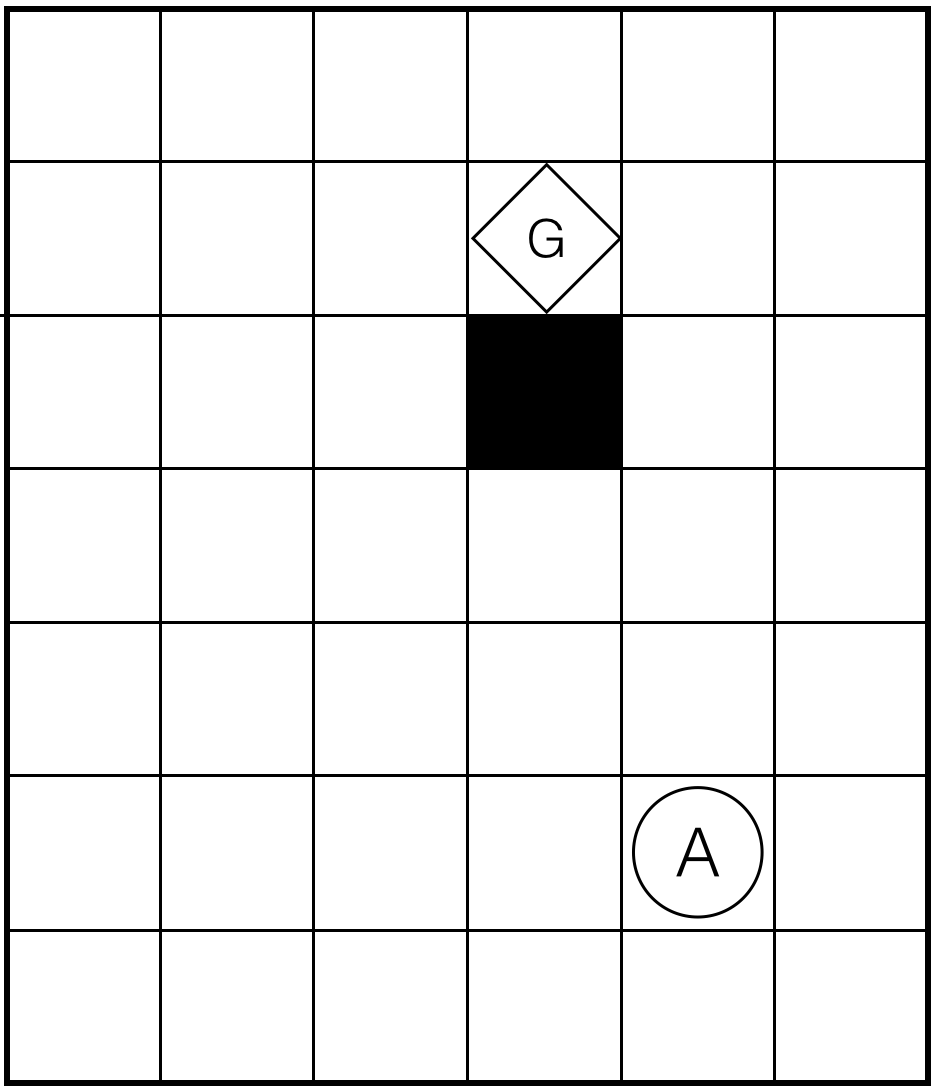
\includegraphics[width=0.32\linewidth]{figures/small_grid.png}}\hspace{10mm}
\subfigure[A large task generated with constraints $\phi_large$]{
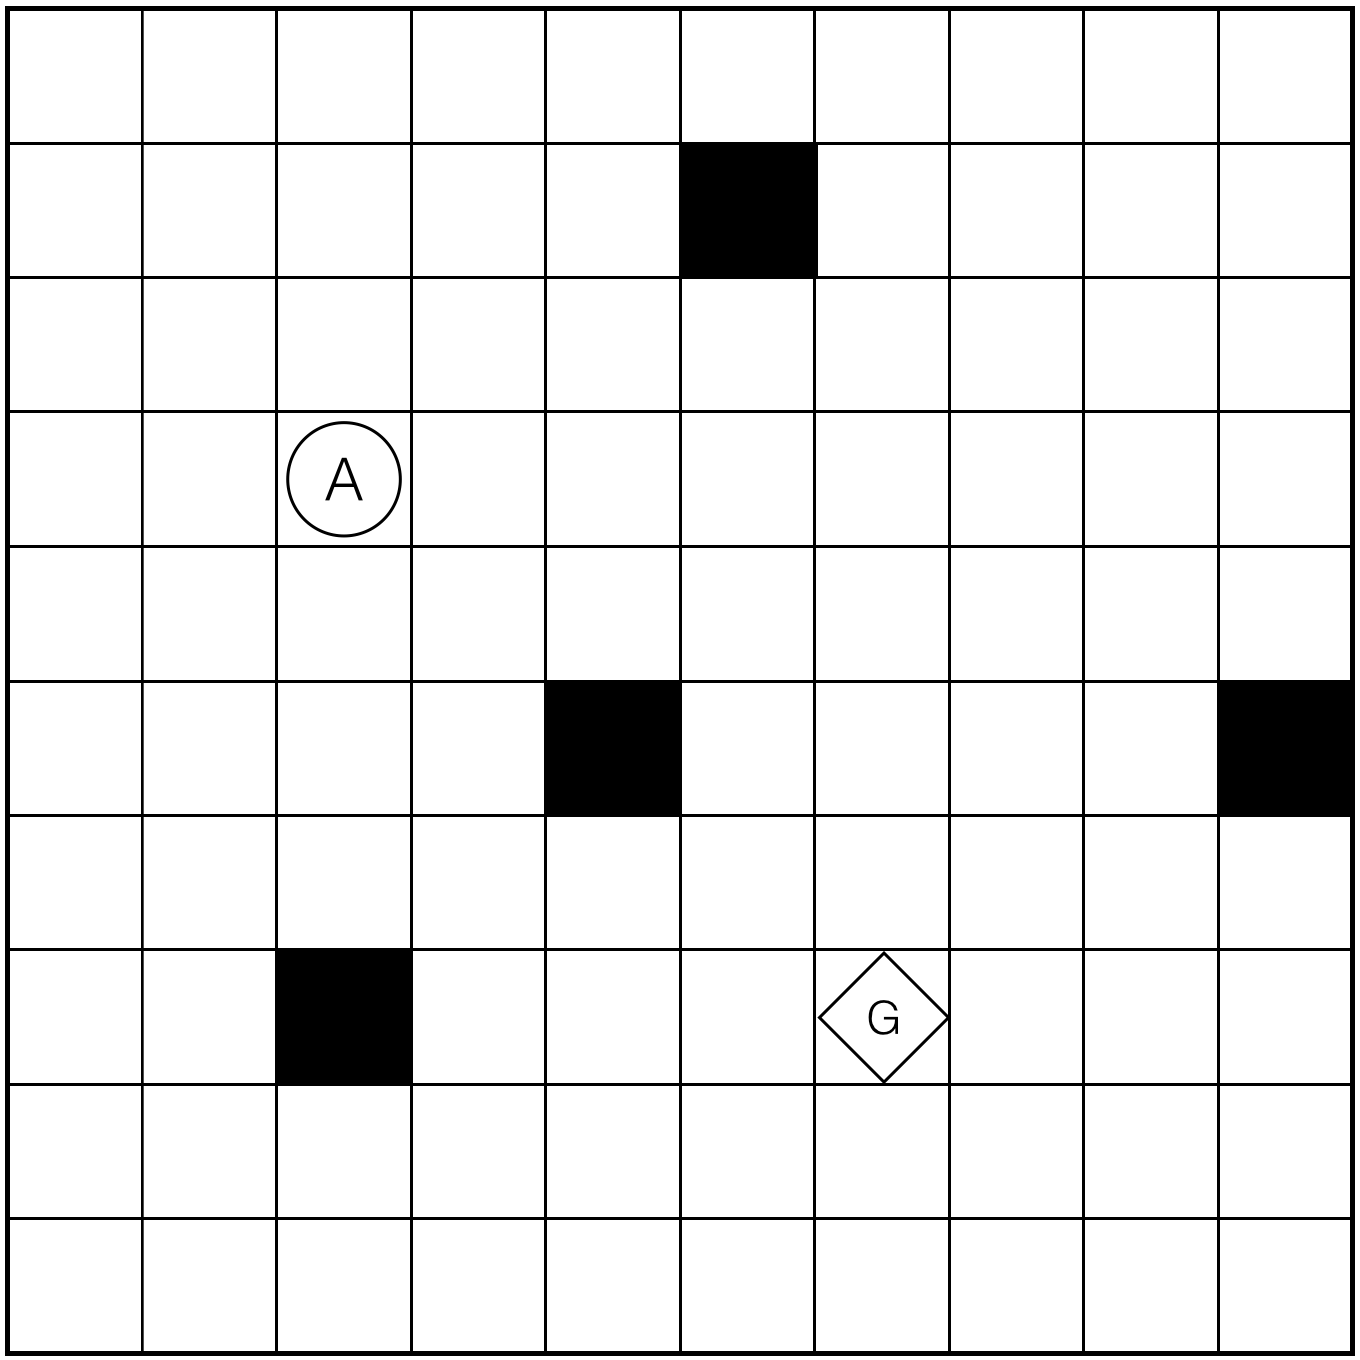
\includegraphics[width=0.32\linewidth]{figures/large_grid.png}}
  \caption{Different randomly generated tasks from the Grid World domain.}
  \label{fig:grid_examples}
\end{figure}

Significantly, the grid world domain $G$ contains infinitely many tasks, since $\textsc{Dom}(c)$ allows for an infinite space of attribute assignments. With a set of constraints, $\phi$, the space is constrained, so there are only finitely many tasks.

Figure~\ref{fig:task_generator} shows the full task generation pipeline. Given a set of constraints, $\phi_{small}$, and a domain $G$, we make three queries to $\Omega$ to generate three tasks, $\tau_1, \tau_2, \tau_3$.

% Task Generator Example
\begin{figure}
\centering
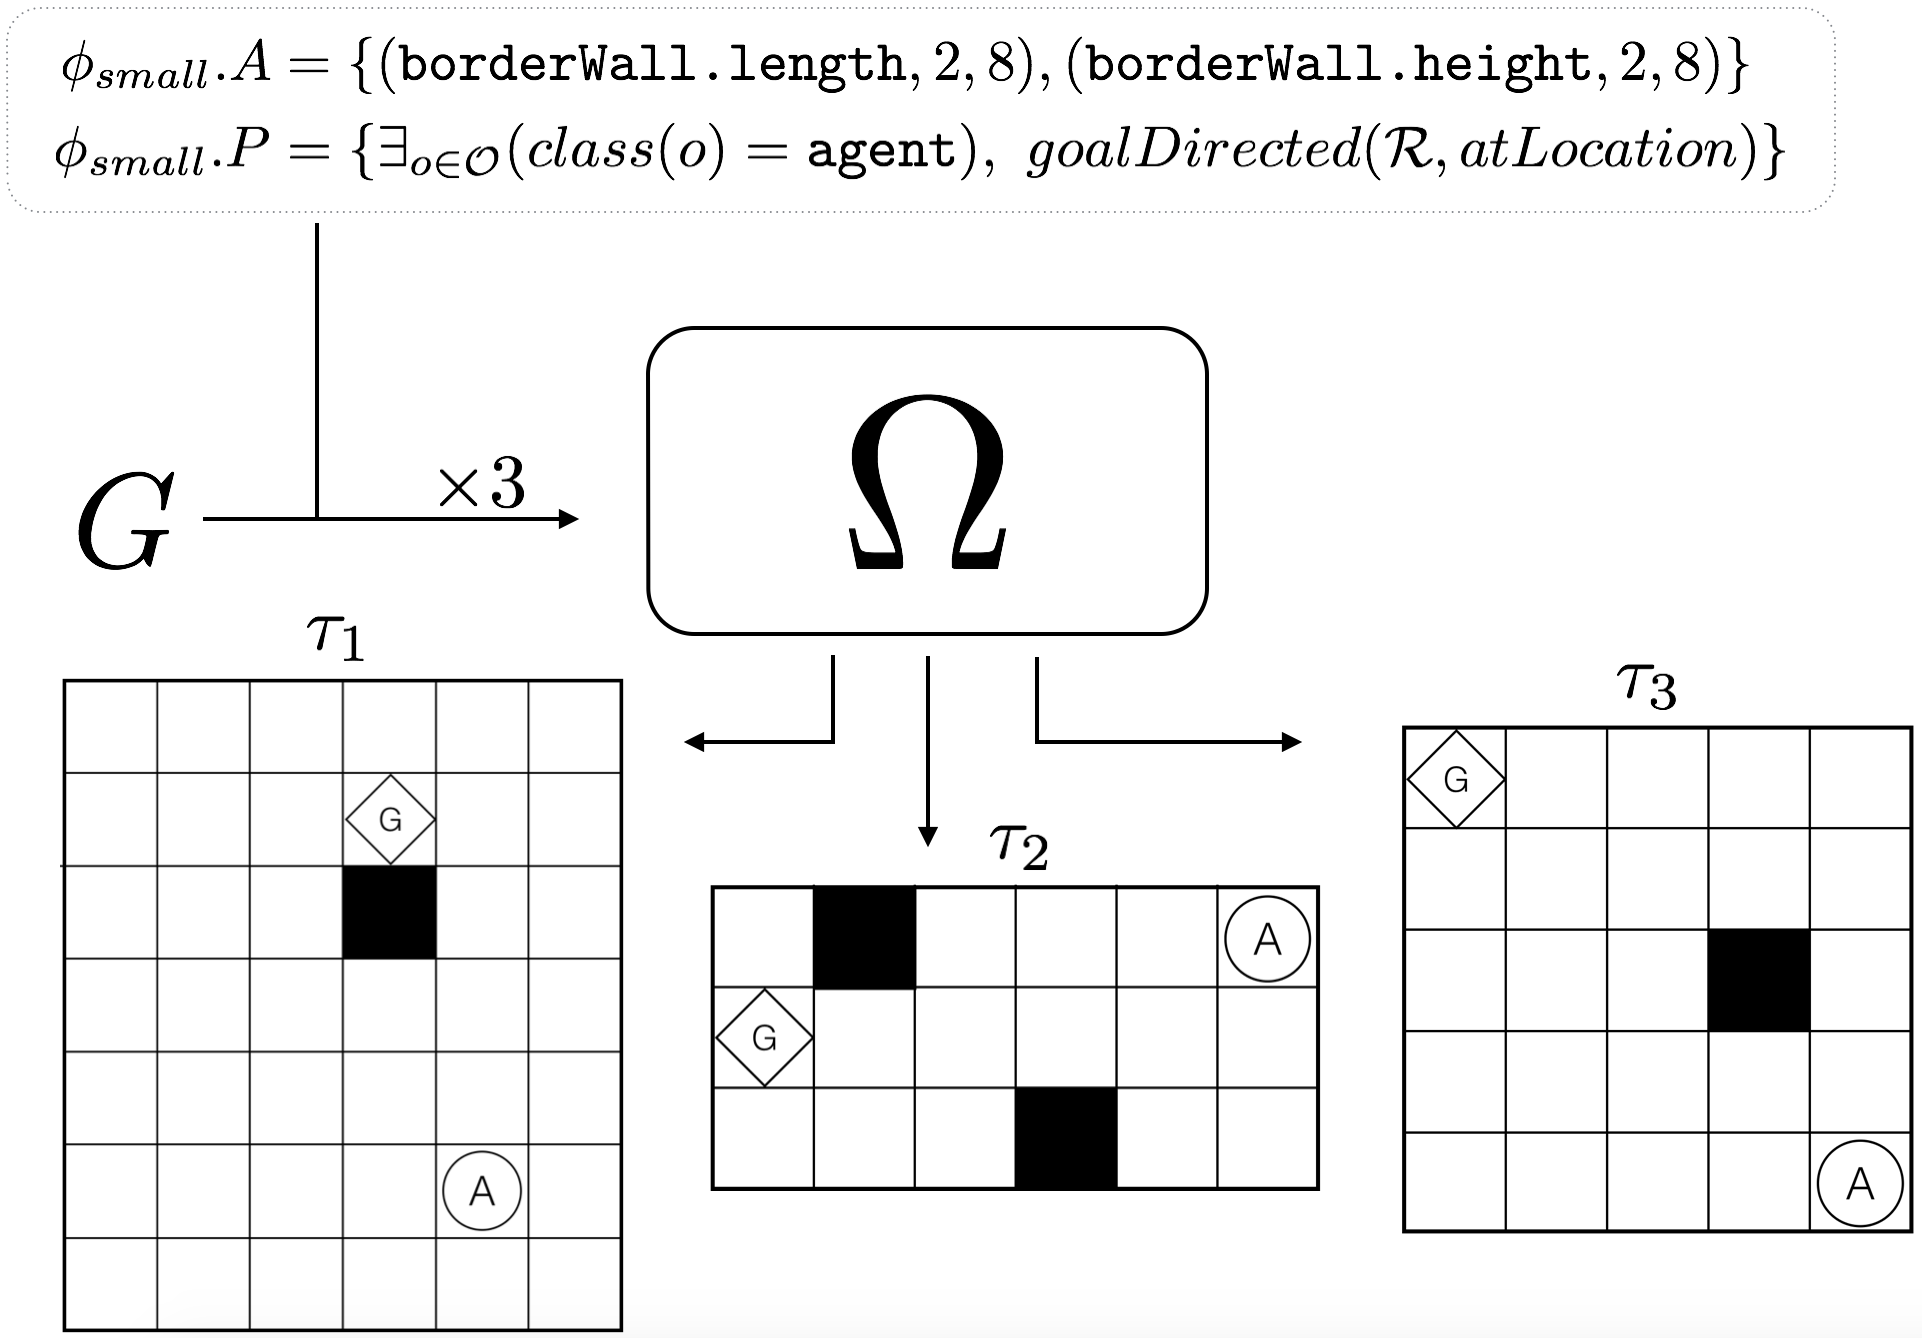
\includegraphics[width=0.7\linewidth]{figures/task_generator.png}
\label{fig:task_generator}
\caption{Three example tasks from the Grid World domain generated by $\Omega$.}
\end{figure}


% Shoutout to PAC.
\subsection{Computational Learning Theory}
Alternatively, we may view a Task Generator instance as a probability distribution over the space of tasks defined by the domain $D$ with respect to the uniform distribution over the constraints $\phi.A$. That is, consider the space of tasks where the constraints $\phi.P$ are all satisfied. Then $\phi.A$ defines the space of possible values for a random variable. This consideration allows interesting extensions to the Probably Approximately Correct framework. Note that different values of $\phi.A$ will lead to two different and possibly disjoint distributions over tasks. This problem structure lets us consider variants to the PAC problem wherein the training distribution is disjoint from the test distribution, but is related in virtue of the tasks belonging to the same domain. ~\cite{baxter2000model} performed a theoretical investigation into the PAC framework where the training and test distributions are disjoint. In future work, we would like to further this investigation in the context of learning to plan.

\subsection{Agent Space}
Consider two tasks $\tau_1$ and $\tau_2$, both belonging to the same domain $D$. The critical observation is that knowledge acquired by solving $\tau_1$, that is, computing the optimal policy $\pi_1$, may be useful when solving $\tau_2$. Consider the case that $\tau_1 = \tau_2$. Then clearly determining the optimal policy for $\tau_2$ is trivial.

Consider that $\tau_1$ and $\tau_2$ both have Goal-Based Reward Functions operating under predicate $p$. Furthermore, since $\tau_1, \tau_2 \in D$, we know that the space of classes, $D.\mathcal{C}$, the action space, transition dynamics, and space of attributes is shared between the two tasks.

Thus, the idea is to use our knowledge of what is shared between two tasks belonging to the same domain in order to {\it translate} between them. Since the both $\tau_1$ and $\tau_2$ share object classes, we know that predicates operating on objects are guaranteed to preserve meaning across tasks. Critically, relations among objects will still be relevant across tasks. For instance, predicates that operate on the attributes of the agent will necessarily transfer between $\tau_1$ and $\tau_2$, assuming these tasks were generated under the constraint that an agent object exists in the task.

One example of knowledge that can be learned from a series of training tasks are {\it goal-based action priors}. These priors are represented in agent space, enabling transfer across tasks from the same domain. Critically, these priors prune away actions on a state by state basis for any task belonging to the target domain, reducing the number of state-action pairs the agent needs to evaluate in order to perform optimally. We now introduce these priors.

% --- Goal-Based Action Priors
\section{Goal-Based Action Priors}
\label{sec:gbaps}

To address state-action space explosions in planning tasks,
we investigate learning an action prior conditioned on the current state and an abstract goal description. This {\it goal-based action prior}
enables an agent to prune irrelevant actions on a
state-by-state basis according to the agent's current goal, focusing the agent on
the most promising parts of the state space. The agent will learn these priors from solving simple task instances and use this knowledge on more complex tasks generated from the same domain.
 
Goal-based action priors can be specified by hand or learned by repeated queries to a Task Generator for a given domain $D$, making them a concise, transferable, and learnable means of
representing useful planning knowledge. 

Our results demonstrate
that these priors provide dramatic improvements for a variety of
planning tasks compared to baselines in simulation, and are applicable
across different tasks.  Moreover, while manually provided
priors outperform baselines on difficult problems, our approach
is able to learn goal-based action priors from experience on simple, tractable, 
training problems that yield even greater performance on the difficult problems
than manually provided priors.

As discussed previously, we conduct experiments in Minecraft. Figure~\ref{fig:example}
shows an example of two problems from the same domain in the game
Minecraft; the agent learns on simple tasks produced by a Task Generator,
(like the problem in the left image) and tests
on new harder problems from the same domain that it has never previously
encountered (like the problem in the right image). All associated code with this paper may be found at
http://h2r.cs.brown.edu/affordances.

\subsection{Approach}
We define a {\it goal-based action prior} as knowledge provided to a planning algorithm to help reduce problem complexity. These priors are used to prune actions on a state by state basis, which naturally reduces the number of state-action pairs the agent needs to evaluate. The key observation is that for action-rich domains (i.e. $\mathcal{A}$ is large), many actions are not relevant in every state, but are still relevant at some point in the task. Using goal-based action priors, an agent will be biased toward the most relevant action applications for each state, encouraging the agent to explore the most promising parts of the state space.

% -- Figure: Minecraft pic --
\begin{figure}[t]
\centering
\subfigure[Mine the gold and smelt it in the furnace]{
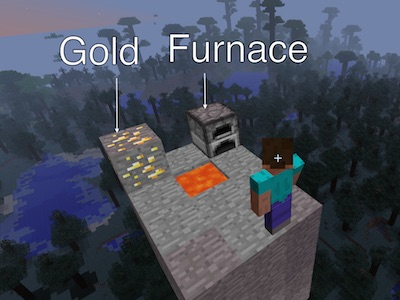
\includegraphics[width=0.3\linewidth]{figures/smelt_scaled_small.jpg}}
\subfigure[Dig down to the gold and mine it, avoiding lava.]{
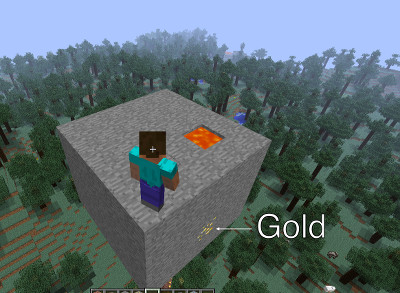
\includegraphics[width=0.3\linewidth]{figures/mining_labeled.jpg}}
\subfigure[Navigate to the goal location, avoiding lava.]{
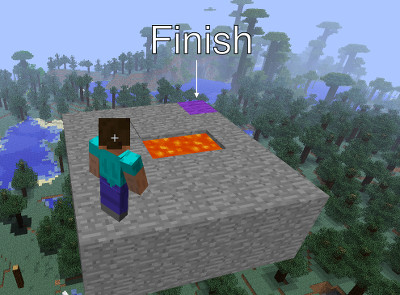
\includegraphics[width=0.3\linewidth]{figures/plane.jpg}}
  \caption{Three different problems from the Minecraft domain.}
  \label{fig:minecraft}
\end{figure}


% -- Subsection: Modeling the Optimal Actions --
\subsection{Modeling the Optimal Actions}

The goal is to formalize planning knowledge that allows an agent to
avoid searching suboptimal actions in each state based on the agent's
current goal. This knowledge must be defined in a way that it is applicable across tasks from the same domain (i.e. in agent space).

First we define the optimal action set, $\mathcal{A}^*$, for a
given state $s$ and goal $G$ as:
% -- Equation: Optimal Action Set --
\begin{equation}
\mathcal{A}^* = \left\{ a \mid Q^*_G(s,a) = V^*_G(s) \right\}, 
\label{eq:opt_act_set}
\end{equation}
where $Q^*_G(s,a)$ and $V^*_G(s)$ represent the optimal Q function and 
value function, respectively.

We learn a probability distribution over the optimality of each action
for a given state ($s$) and goal ($G$). Thus, we want to infer a Bernoulli
distribution for each action's optimality:
% -- Equation: Master Equation --
\begin{equation}
\Pr(a_i \in \mathcal{A}^* \mid s, G)
\label{eq:master}
\end{equation}

\noindent for $i \in \{1, \ldots, |\mathcal{A}|\}$, where
$\mathcal{A}$ is the OO-MDP action space for the domain.

To generalize across tasks, we abstract the state
and goal into a set of $n$ paired predicates and goals, $\{
(p_1, g_1) \ldots (p_{n}, g_{n}) \}$. We abbreviate each pair $(p_j,
g_j)$ to $\delta_j$ for simplicity. Each predicate is an agent space predicate, $p \in
\mathcal{P_agent}$ ensuring transferability between tasks, and $G$ is a {\it goal} which is a
predicate on states that is true if and only if a state is terminal. For example, a
predicate might be $nearTrench(agent)$ which is true when the agent is
standing next to a trench object.  In general these could be arbitrary
logical expressions of the state; in our experiments we used unary
predicates. A goal specifies the sort of problem the agent is trying to solve, such as the agent
retrieving an object of a certain type from the environment, reaching
a particular location, or creating a new structure.  Depending on the
agent's current goal, the relevance of each action changes
dramatically.  We rewrite Equation~\ref{eq:master}:
% -- Equation: replace K --
\begin{equation}
\Pr(a_i \in \mathcal{A}^* \mid s, G) = \Pr(a_i \in \mathcal{A}^* \mid s, G, \delta_1 \ldots \delta_n).
\end{equation}

We introduce the indicator function $f$, which returns 1 if and only if the given $\delta$'s predicate is true in the provided state $s$, and $\delta$'s goal is entailed by the agent's current goal, $G$:
% -- Equation: function f defn --
\begin{equation}
f(\delta, s, G) = 
\begin{cases}
1& \delta.p(s) \wedge \delta.g(G) \\
0& \text{otherwise.}
\end{cases}
\label{eq:f_func_def}
\end{equation}

Evaluating $f$ for each $\delta_j$ given the current state and goal gives rise to a set of binary features,
$\phi_j = f(\delta_j, s, G)$, which we use to reformulate our probability distribution:
% -- Equation: Master Equation --
\begin{equation}
\Pr(a_i \in \mathcal{A}^*  \mid s, G, \delta_1 \ldots \delta_n) = \Pr(a_i \in \mathcal{A}^*  \mid \phi_1, \ldots, \phi_n)
\label{eq:feature_rep}
\end{equation}

This equation models how optimal each action is given a state, and goal. Critically, we can rewrite the lefthand side of the equation in terms of $\phi_1, \ldots, \phi_n$, which provides an agent space representation of the current state. This intermediary representation is exactly what enables our agent to transfer these priors from a set of training tasks to an arbitrary task from the same domain.

This distribution may be modeled in a number of ways, making this approach extremely flexible.

% Expert Model
\subsubsection{Expert Model} One model that can be specified by
an expert is an OR model.
In the OR model some subset of the features 
($\phi^i \subset \phi$) are
assumed to cause action $a_i$ to be optimal; as long as one of
the features is on, the probability that $a_i$ is optimal is one.
If none of the features are on, then the probability that $a_i$ is 
optimal is zero. More formally,
\begin{equation}
\Pr(a_i \in \mathcal{A}^*  \mid \phi_1, \ldots, \phi_n) = \phi_1^i \lor ... \lor \phi_m^i,
\end{equation}
where $m$ is the number of features that can cause $a_i$ to be optimal ($m = |\phi^i|$).

In practice, we do not expect such a distribution to be reflective of
reality; if it were, then no planning would be needed because a full
policy would have been specified. However, it does provide a
convenient way for a designer to provide conservative background
knowledge. Specifically, a designer can consider each precondition-goal
pair and specify the actions that could be optimal in that context, ruling
out actions that would be known to be irrelevant or dependent on other
state features being true.

Because the OR model is not expected to be reflective of
reality and because of other limitations (such as not allowing support
for an action to be provided when a feature is off), the model is not
practical for learning.

% Learned Priors
Our real goal is to learn from a series of simple tasks, and use this knowledge to solve much more challenging problems. Again, this strategy is heavily inspired by the notion of scaffolding discussed earlier.

Furthermore, learned priors have the potential to outperform
hand-coded priors by more flexibly adapting to the
features that predict optimal actions over a large training set.
We consider two models, Naive Bayes and Logistic Regression.

\subsubsection{Naive Bayes}
An alternative more expressive model that does lend itself to learning is
Naive Bayes. We first factor using Bayes' rule, introducing a parameter vector $\theta_i$ of
feature weights:

% -- Equation: Bayes --
\begin{equation}
\Pr(a_i \in \mathcal{A}^*  \mid \phi_1, \ldots, \phi_n) = \frac{\Pr(\phi_1, \ldots, \phi_{n}, \mid a_i \in \mathcal{A}^*, \theta_i) \Pr(a_i \in \mathcal{A}^* \mid \theta_i)}{\Pr(\phi_1, \ldots, \phi_{n} \mid \theta_i)}
\label{eq:bayes}
\end{equation}

Next we assume that each feature is conditionally independent of the others, given whether the action is optimal:
% -- Equation: Naive assumption and uniform prior--
\begin{equation}
= \frac{\prod_{j=1}^{n} \Pr(\phi_j \mid a_i \in \mathcal{A}^*, \theta_i) \Pr(a_i \in \mathcal{A}^* \mid \theta_i) }{\Pr(\phi_1, \ldots, \phi_{n} \mid \theta_i)}
\label{eq:final}
\end{equation}

Finally, we define the prior on the optimality of each action to be
the fraction of the time each action was optimal during training.

\subsubsection{Logistic Regression}

In Logistic Regression, classification is computed by a logistic threshold function. That is, a vector of weights $\vec{w}$ is learned that determines the optimal decision boundary:
\begin{equation}
\textsc{LogReg}(s) = \frac{1}{1 + e^{-\vec{w} \cdot \phi(s)}}
\end{equation}

Where $\phi(s)$ denotes the agent space features extracted from the state $s$ introduced above. Then, our decision rule for classification is simply:
\begin{equation}
\begin{cases}
1&\textsc{LogReg}(s) \geq 0.5 \\
0&\text{otherwise}
\end{cases}
\end{equation}

% -- Subsection: Learning the Optimal Actions--
\subsection{Learning the Optimal Actions}
For learning we consider a Task Generator $\Omega$, a domain $D$, and a set of constraints, $\phi_{\textsc{Train}}$. These constraints will force the tasks output by $\Omega$ to be sufficiently small (i.e. small enough so that tabular approaches like Value Iteration can solve for the optimal policy).

We generate $n$ training tasks, $\tau_1, \ldots, \tau_n$, and solve for the optimal policy in each task, $\pi_1, \ldots, \pi_n$.

Using the optimal policies across these tasks, we can learn the model parameters for the Naive Bayes model, or inform the weights for the Logistic Regression model.

To compute model parameters using Naive Bayes, we compute
the maximum likelihood estimate of the parameter vector $\theta_i$ for
each action using the policy.

Under our Bernouli Naive Bayes model, we estimate the parameters
$\theta_{i,0} = \Pr(a_i)$ and $\theta_{i,j} = \Pr(\phi_j | a_i)$, for $j \in \{1, \ldots, n \}$, where the maximum likelihood estimates are:
\begin{align}
\theta_{i,0} &= \frac{C(a_i)}{C(a_i) + C(\bar{a_i})} \\
\theta_{i,j} &= \frac{C(\phi_j, a_i)}{C(a_i)}
\end{align}

Here, $C(a_i)$ is the number of observed occurrences where $a_i$ was optimal across all worlds $W$,
$C(\bar{a_i})$ is the number of observed occurrences where $a_i$ was not optimal,
and $C(\phi_j, a_i)$ is the number of occurrences where $\phi_j=1$ and $a_i$ was optimal.
We determined optimality using the synthesized policy for each training world, $\pi_w$. More formally:

\begin{align}
C(a_i) &= \sum_{w \in W} \sum_{s \in w} (a_i \in \pi_w(s)) \\
C(\bar{a_i}) &= \sum_{w \in W} \sum_{s \in w} (a_i \not \in \pi_w(s) ) \\
C(\phi_j, a_i) &= \sum_{w \in W} \sum_{s \in w} (a_i  \in \pi_w(s) \wedge \phi_j == 1)
\end{align}

To compute the optimal decision boundary for Logistic Regression, we compute gradient descent using the $L_2$ loss function, resulting in the following update rule:

\begin{equation}
w_i \leftarrow w_i + \alpha(y - \textsc{LogReg}(s)) \times \textsc{LogReg}(s)(1 - \textsc{LogReg}(s))
\end{equation}

We optimize until convergence.

During the learning phase, the agent learns when actions are useful
with respect to the agent space features.  For example, consider the three different
problems shown in Figure~\ref{fig:minecraft}.  During training, we observe
that the \texttt{destroy} action is often optimal when the agent is
looking at a block of gold ore and the agent is trying to smelt gold
bars.  Likewise, when the agent is not looking at a block of gold
ore in the smelting task we observe that the \texttt{destroy} action
is generally not optimal (i.e. destroying grass blocks is typically
irrelevant to smelting).  This information informs the distribution
over the optimality of the \texttt{destroy} action, which is used at
test time to encourage the agent to destroy blocks when trying to
smelt gold and looking at gold ore, but not in other situations
(unless the prior suggests using \texttt{destroy}). Example
learned priors are shown in~\ref{fig:example_affs}.

% Sample priors
\begin{figure}
\centering
\subfigure[agentLookTowardGoal]{
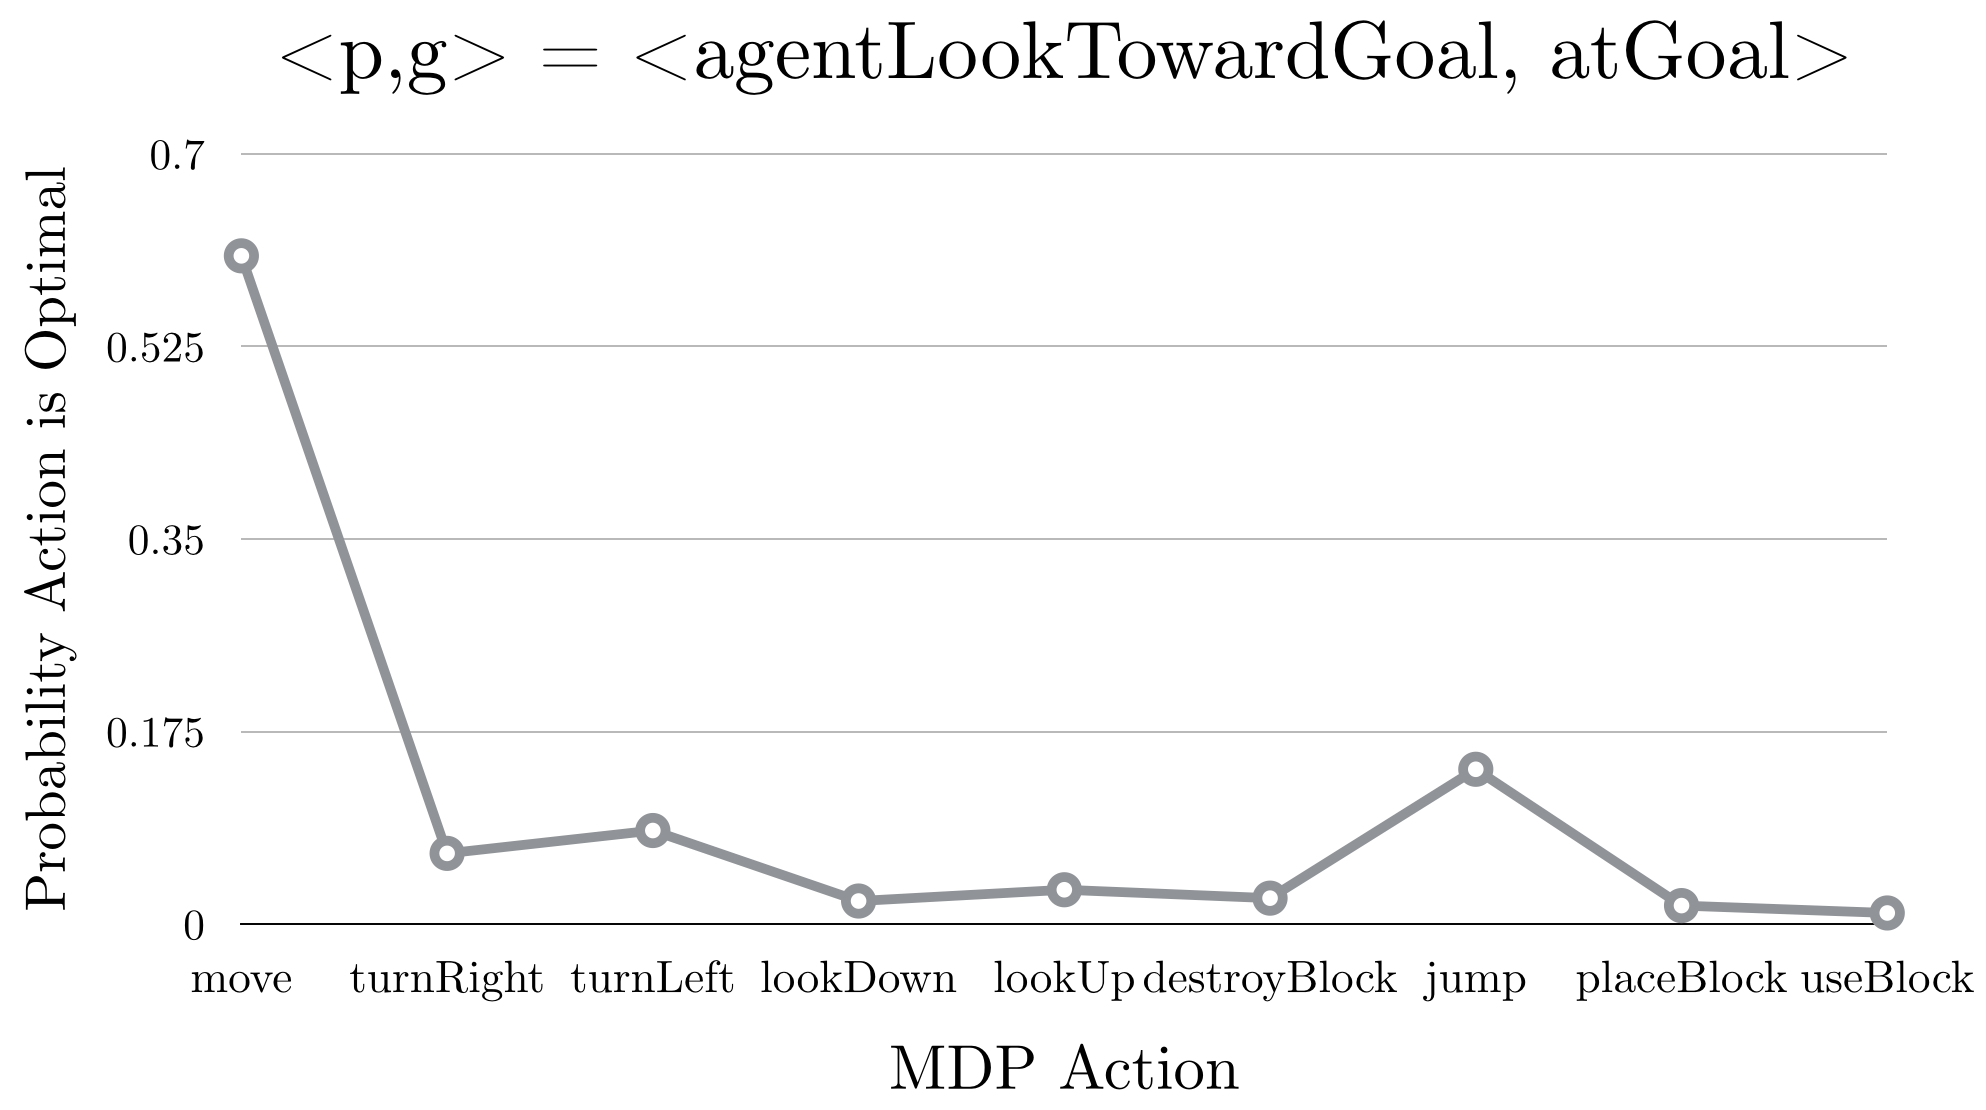
\includegraphics[scale=0.17]{figures/plane_aff.png}}
\subfigure[trenchInFrontOfAgent]{
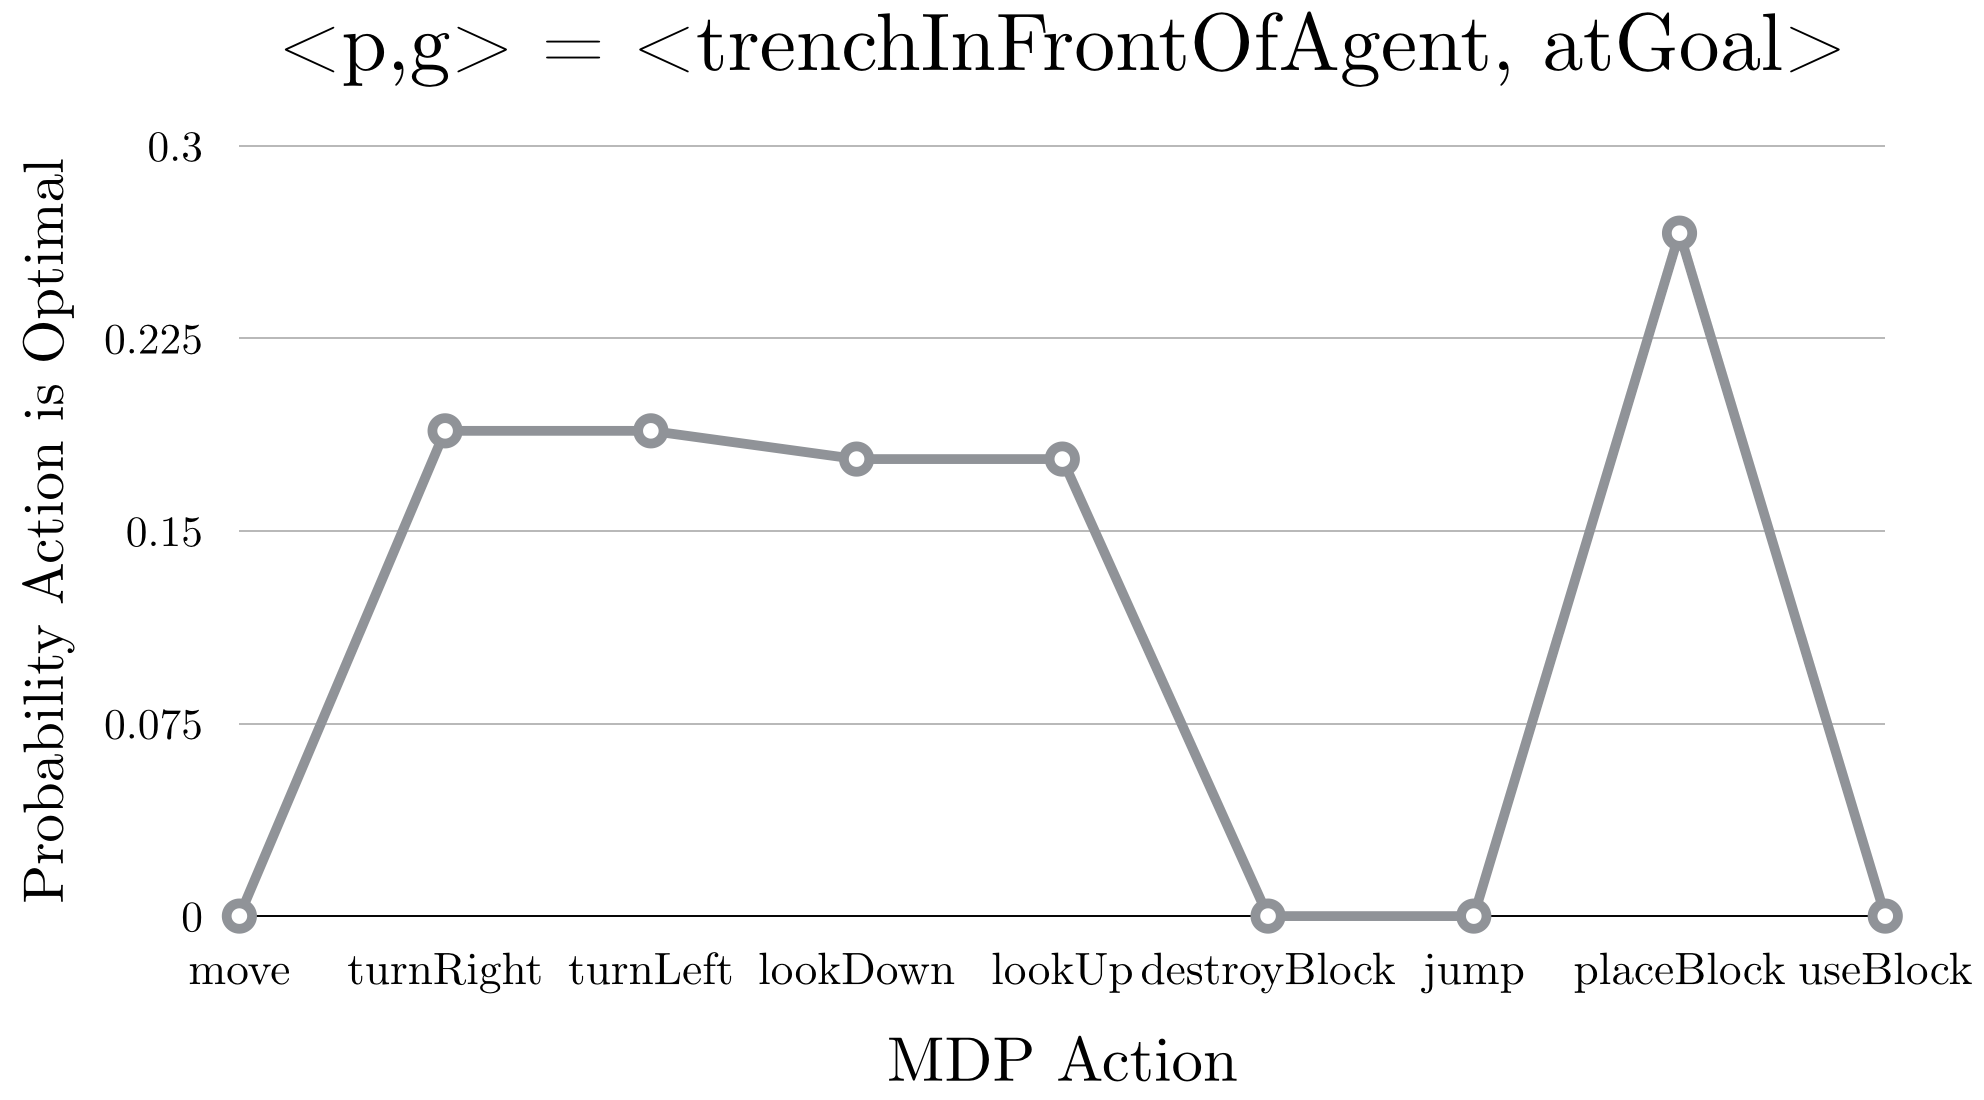
\includegraphics[scale=0.17]{figures/trench_aff.png}}
\label{fig:example_affs}
\caption{When the agent is looking toward its goal location, it is generally better to move forward than do anything else. Alternatively, when the agent is faced with a trench, the agent should walk along the trench to look for gaps, or build a bridge across by looking down and placing blocks.}
\end{figure}

At test time, we query $\Omega$ with a different set of constraints, $\phi_{\textsc{Test}}$ but the same domain $D$. Notably, $\phi_{\textsc{Test}}$ will necessitate larger, more complicated tasks than those trained on. For simplicity, our learning process uses a strict separation between training and test; after learning is complete our model parameters/weights remain fixed.

% -- Subsection: Action Pruning --
\subsection{Action Pruning with Goal-Based Action Priors}
\label{sec:action_pruning}
A planner using a goal-based action prior will prune actions on a state-by-state basis. 

Under the expert specified OR model, when $\Pr(a_i \in \mathcal{A}^*  \mid \phi_1, \ldots, \phi_n) = 0$
action $a_i$ is pruned from the planner's consideration. When
$\Pr(a_i \in \mathcal{A}^*  \mid \phi_1, \ldots, \phi_n) = 1$,
action $a_i$ remains in the action set to be searched by the planner.

% What to do with logreg/naive bayes
Under Naive Bayes, we found that the optimal decision rule resulted in poor performance as a consequence of pruning away too many actions. Instead, we imposed a more conservative threshold, only pruning away actions if they were extremely unlikely to be sub-optimal.

Under Logistic Regression, we used the optimal decision rule to determine which actions were to be considered in each state.

% -- Subsection: Analysis --
\subsection{Analysis}

% -- EVALUATION --
\section{Evaluation}
\label{sec:evaluation}

We evaluate our approach using the game Minecraft. Minecraft is a 3D blocks game in which the
user can place, craft, and destroy blocks of different types.
Minecraft's physics and action space allow users to create complex
systems, including logic gates and functional scientific graphing
calculators.

Minecraft is a voxel-based simulation in which the user-controlled agent can place, craft, and destroy blocks of different types.
Minecraft's physics and action space are extremely expressive and allow users to create complex objects and systems, including logic gates and functional scientific graphing calculators.
Minecraft serves as a model for complicated real world systems such as robots traversing complex terrain, and large scale construction projects involving highly malleable environments.  As in these tasks, the agent operates in a very large state-action space in an uncertain environment. Figure~\ref{fig:minecraft} shows three example scenes from Minecraft problems that we solve.

%Additionally, we used expert-provided priors to
%enable a manipulator robot to infer helpful actions in response to a
%person working on a kitchen task, shown in Figure~\ref{fig:baxter_results}.


\subsection{Experiments}
Our experiments consist of five common tasks in Minecraft:
bridge construction, gold smelting, tunneling through
walls, digging to find an object, and path planning.

% TRAINING
The training set consists of 20 randomly generated tasks for each goal, for a total of 100 instances. Each instance is extremely simple: 1,000-10,000 states (small enough to solve with tabular approaches). The output of our training process is the model parameter $\theta$ or the weight vector $\vec{w}$, which inform our goal-based action prior depending on which model we are using. The full training process takes approximately one hour run in parallel on a computing grid, with the majority of time devoted to computing the optimal value function for each training instance.

% TEST
The test set consists of 20 randomly generated tasks from the same domain, with the same five goals, for a total of 100 instances. Each instance is extremely complex: 50,000-1,000,000 states (which is far too large to solve with tabular approaches).

We fix the number of features at the start of training based on the number
predicates defined by the OO-MDP, $|\mathcal{P}|$, and the number of goals, $|G|$.
We provide our system with a set of 51 features that are likely to aid in predicting the correct action across instances.

We use Real-Time Dynamic Programming (RTDP)~\cite{barto95} as our
baseline planner, a sampling-based algorithm that does not require the
planner to exhaustively explore states. We compare RTDP with
priors learned under Naive Bayes used in RTDP (LP-RTDP), and expert priors RTDP (EP-RTDP).
We terminate each planner when the maximum change in
the value function is less than 0.01 for 100 consecutive policy
rollouts, or the planner fails to converge after 1000 rollouts.  The
reward function is $-1$ for all transitions, except transitions to
states in which the agent is in lava, where we set the reward to
$-10$. The goal specifies terminal states, and the discount factor is
$\gamma = 0.99$.  To introduce non-determinism into our problem,
movement actions (move, rotate, jump) in all experiments have a small
probability (0.05) of incorrectly applying a different movement
action.  This noise factor approximates noise faced by a physical
robot that attempts to execute actions in a real-world domain and
can affect the optimal policy due to the existence of lava pits

We report the number of Bellman updates executed by each planning
algorithm, the accumulated reward of the average plan, and the CPU
time taken to find a plan. Table~\ref{table:minecraft_results} shows
the average Bellman updates, accumulated reward, and CPU time for
RTDP, LP-RTDP and EP-RTDP after planning in 20 different maps of each
goal (100 total). Figure~\ref{fig:average_results} shows the
results averaged across all maps.  We report CPU time for
completeness, but our results were run on a networked cluster where
each node had differing computer and memory resources. As a result,
the CPU results have some variance not consistent with the number of
Bellman updates in Table~\ref{table:minecraft_results}.  Despite this
noise, overall the average CPU time shows statistically significant
improvement overall with our priors, as shown in
Figure~\ref{fig:average_results}. Furthermore, we reevaluate each
predicate every time the agent visits a state, which could be optimized by caching predicate evaluations, further
reducing the CPU time taken for EP-RTDP and LP-RTDP.

\subsection{Results}

% -- Table: Minecraft Naive Bayes results --
\begin{table}
\centering
\ra{1.15}
\small
\begin{tabular}{@{}llll@{}}\toprule
Planner & Bellman & Reward & CPU \\ \midrule
&\hspace{-10mm}{\it Mining Task} \\
\texttt{RTDP} & 17142.1 ($\pm$3843) 		& {\bf -6.5} ($\pm$1)  & {\bf 17.6s}   ($\pm$4) \\
\texttt{EP-RTDP} 	& 14357.4 ($\pm$3275) 		& {\bf -6.5}   ($\pm$1) & 31.9s   ($\pm$8) \\
\texttt{LP-RTDP} 	& {\bf 12664.0} ($\pm$9340) 	& -12.7 ($\pm$5) & 33.1s   ($\pm$23) \\\hline
&\hspace{-10mm}{\it Smelting Task} \\
\texttt{RTDP} 	& 30995.0 ($\pm$6730) 		& {\bf -8.6}   ($\pm$1) & 45.1s   ($\pm$14) \\
\texttt{EP-RTDP} 	& 28544.0 ($\pm$5909) 		& {\bf -8.6}   ($\pm$1) & 72.6s   ($\pm$19) \\ 
\texttt{LP-RTDP} 	& {\bf 2821.9} 	 ($\pm$662) 	& -9.8   ($\pm$2) & {\bf 7.5s}  ($\pm$2) \\ \hline
&\hspace{-10mm}{\it Wall Traversal Task} \\
\texttt{RTDP} & 45041.7 ($\pm$11816) 		& -56.0   ($\pm$51) & {\bf 68.7s}   ($\pm$22) \\
\texttt{EP-RTDP} 	& 32552.0 ($\pm$10794) 		& -34.5   ($\pm$25) & 96.5s   ($\pm$39) \\ 
\texttt{LP-RTDP} 	& {\bf 24020.8} ($\pm$9239) 	& {\bf -15.8}   ($\pm$5) & 80.5s   ($\pm$34) \\ \hline
&\hspace{-10mm}{\it Trench Traversal Task} \\
\texttt{RTDP}  	& 16183.5 ($\pm$4509) 		& {\bf -8.1}   ($\pm$2) & 53.1s   ($\pm$22) \\
\texttt{EP-RTDP} 	& {\bf 8674.8} 	($\pm$2700) 	& -8.2   ($\pm$2) & {\bf 35.9s}   ($\pm$15) \\ 
\texttt{LP-RTDP} 	& 11758.4 ($\pm$2815) 		& -8.7   ($\pm$1) & 57.9s   ($\pm$20) \\ \hline
&\hspace{-10mm}{\it Plane Traversal Task} \\
\texttt{RTDP} & 52407 ($\pm$18432) 		& -82.6   ($\pm$42) & 877.0s   ($\pm$381) \\
\texttt{EP-RTDP} 	& 32928 ($\pm$14997) 		& -44.9   ($\pm$34) & 505.3s   ($\pm$304) \\
\texttt{LP-RTDP} 	& {\bf 19090} 	 ($\pm$9158) 	& {\bf-7.8}   ($\pm$1) & {\bf 246s}  ($\pm$159) \\
\bottomrule
\end{tabular}
\caption{RTDP vs. EP-RTDP vs. LP-RTDP}
\label{table:minecraft_results}
\end{table}

% -- Figure: Average results --
\begin{figure}[t]
%\begin{figure}
\centering
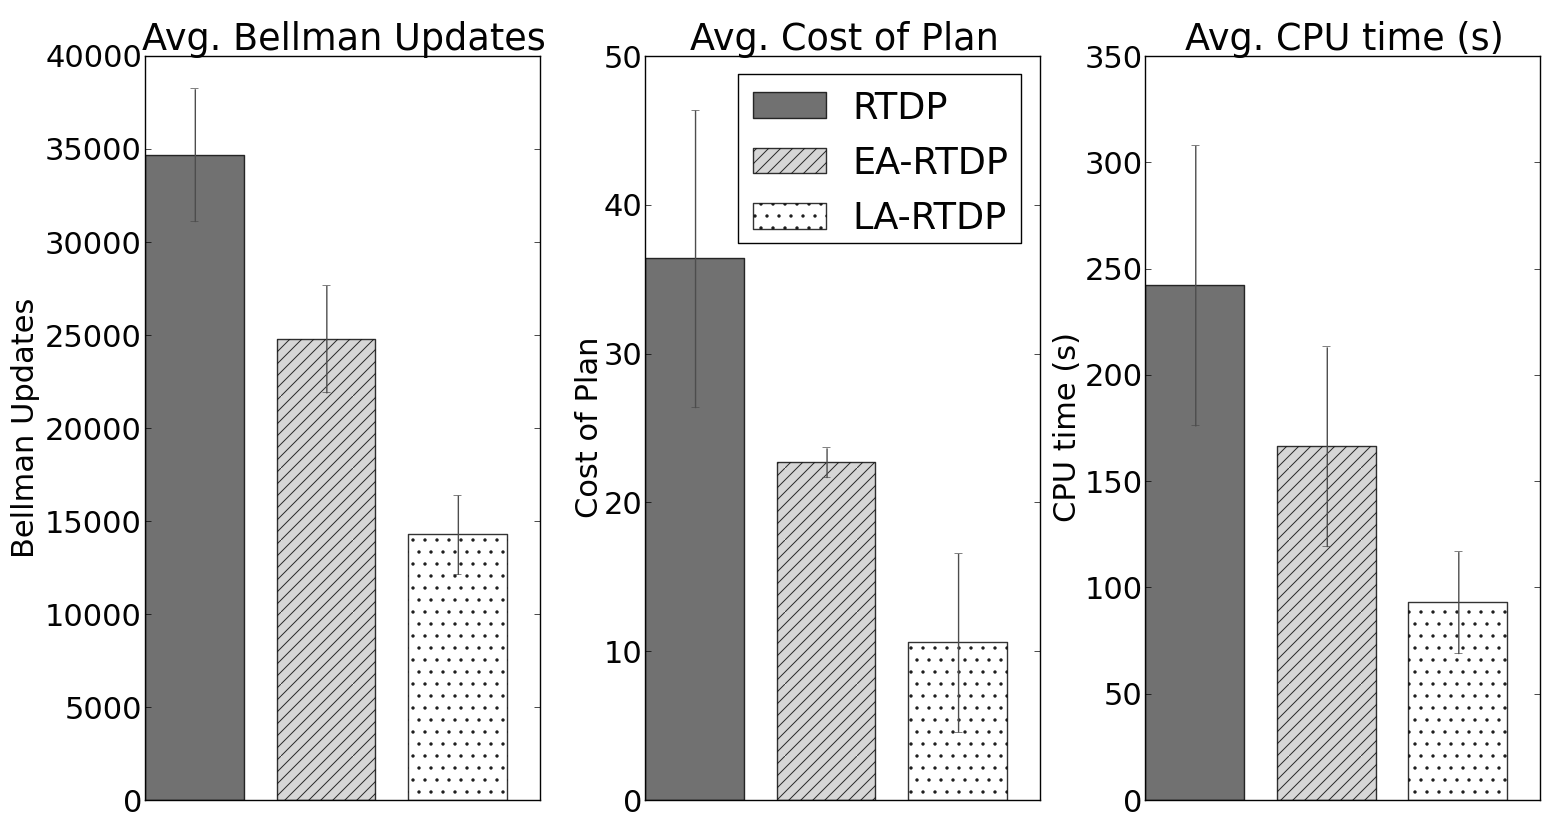
\includegraphics[width=1\linewidth]{figures/average_results_cropped.png}%
%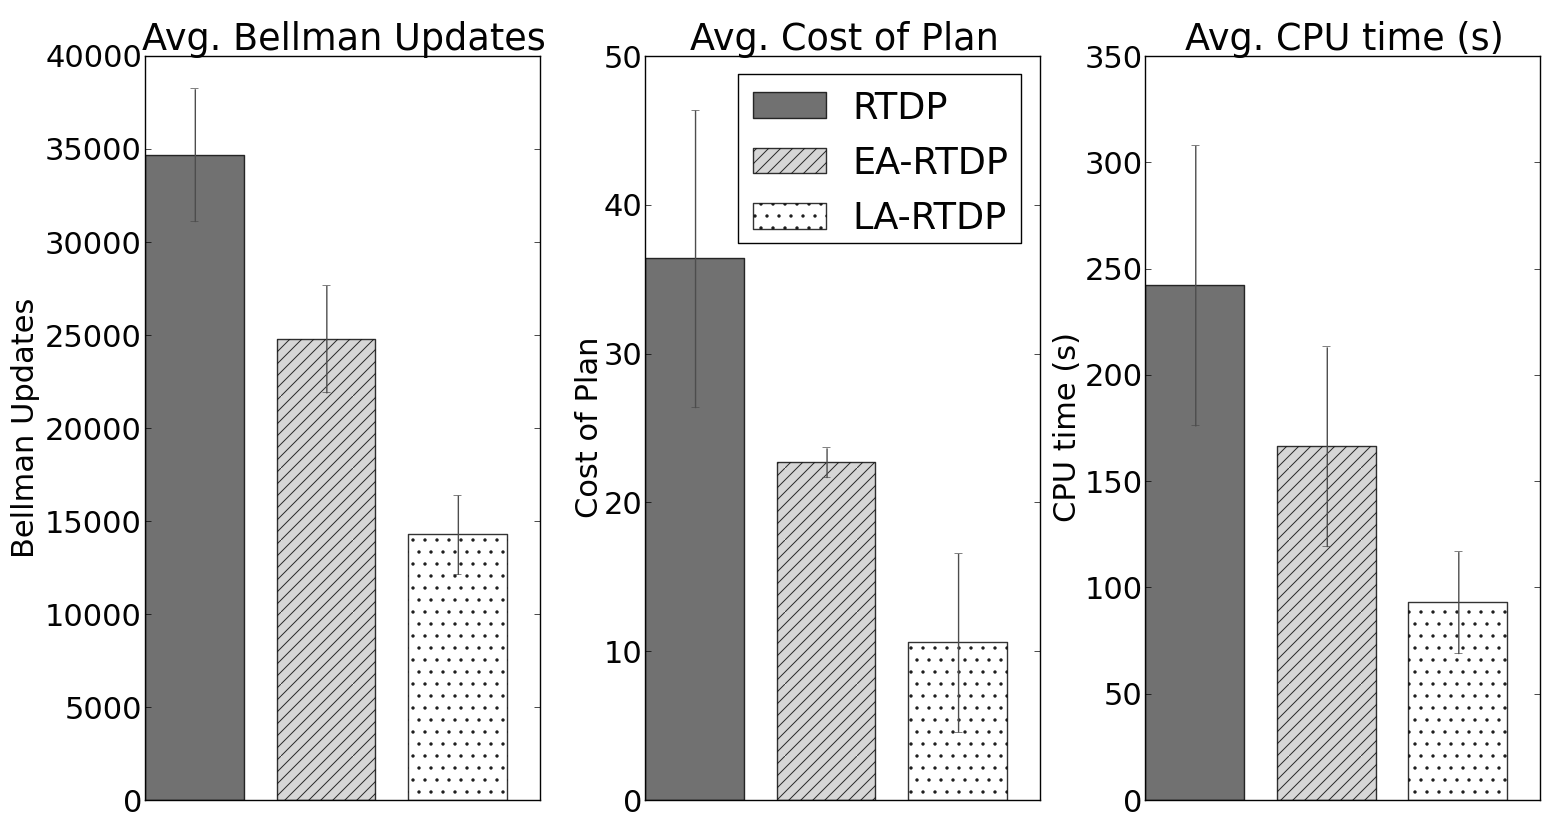
\includegraphics[scale=0.18]{figures/average_results_cropped.png}%
\caption{Average results from all maps.}
\label{fig:average_results}
\end{figure}
%\end{figure}

Because the planners terminate after a maximum of 1000
rollouts, they do not always converge to the optimal policy. LP-RTDP on
average finds a comparably better plan (10.6 cost) than EP-RTDP (22.7
cost) and RTDP (36.4 cost), in significantly fewer
Bellman updates (14287.5 to EP-RTDP's 24804.1 and RTDP's 34694.3), and in
less CPU time (93.1s to EP-RTDP's 166.4s and RTDP's 242.0s).  These
results indicate that while learned priors provide the largest
improvements, expert-provided priors can also significantly
enhance performance. Depending on the domain, expert-provided priors can add
significant value in making large state spaces tractable without the
overhead of supplying training worlds.

For some task types, LP-RTDP finds a slightly worse plan on average than
RTDP ({\em e.g.} the mining task). This worse convergence is due to the fact that LP-RTDP
occasionally prunes actions that are in fact optimal (such as
pruning the \texttt{destroy} action in certain states of the mining task).
%To fix this, we could lower the threshold to allow for even more conservative action pruning. In future work, we plan on investigating approaches
%to dynamically adjusting the threshold based on planning feedback. 
Additionally, RTDP occasionally achieved a faster clock time because EP-RTDP and LP-RTDP also evaluate several OO-MDP predicates in every state, adding a small amount of time to planning.

\subsubsection{Logistic Regression Results}
We conducted similar experiments comparing the Logistic Regression model to Bounded RTDP. In these experiments, we provided a smaller feature set, and only tested on a single goal type. These experiments were conducted as a proof of concept to verify that Logistic Regression can effectively learn useful priors.

In particular, we evaluated on significantly larger tasks than with Naive Bayes. The training tasks are each of a similar size - roughly 1,000-10,000 states. The test tasks are all larger than 1,000,000 states, with several approaching 10,000,000. Each task was provided a goal-directed reward function, defined by the predicate that evaluates whether an agent is at a particular coordinate of the world. In other words, these tasks were large obstacle courses. Lava was scattered randomly throughout the world, and the agent was given blocks to plug up the lava if it desired (one could imagine cases where this is optimal behavior). We conducted tests on 20 randomly generated tasks.

The results are summarized in Table~\ref{table:log_reg_results}. Here we see that in these much larger worlds, 

\begin{table}
\centering
\ra{1.1}
\small
\begin{tabular}{@{}llll@{}}\toprule
Planner & Bellman & Reward & CPU \\ \midrule
\texttt{BRTDP}   			&	40800 ($\pm$2348)		&	-135.3 ($\pm$9)		& 573.6 ($\pm$33) \\
\texttt{LR-BRTDP} 			& 	{\bf 18770} ($\pm$1031)	&	{\bf -15.0} ($\pm$1)& {\bf 129.6} ($\pm$5) \\ \hline
\end{tabular}
\caption{Logistic Regression GBAPs vs. Bounded-RTDP}
\label{table:log_reg_results}
\end{table}

% Need an image.

\subsubsection{Temporally Extended Actions and Goal-Based Action Priors}

The primary defect with including temporally extended actions in the action space is that the branching factor increases, consequently increasing planning time. With the use of goal-based action priors, the agent will learn to prune away irrelevant action applications, including options and macro actions. As a result, goal-based action priors and temporally extended actions are quite complementary.

\begin{table}
\centering
\ra{1.1}
\small
\begin{tabular}{@{}llll@{}}\toprule
Planner & Bellman & Reward & CPU \\ \midrule
\texttt{RTDP}   			&	27439 ($\pm$2348)		&	-22.6 ($\pm$9)		& 107 ($\pm$33) \\
\texttt{LP-RTDP} 			& 	{\bf 9935} ($\pm$1031)	&	{\bf -12.4} ($\pm$1)& {\bf 53} ($\pm$5) \\ \hline
\texttt{RTDP+Opt}  		&	26663 ($\pm$2298)		&	-17.4 ($\pm$4) 		& 129($\pm$35) \\
\texttt{LP-RTDP+Opt} 		& 	{\bf 9675} ($\pm$953)	&	{\bf -11.5} ($\pm$1)	&{\bf 93} ($\pm$10) \\ \hline
\texttt{RTDP+MA}  		&	31083 ($\pm$2468)		&	-21.7	 ($\pm$5)		&336 ($\pm$28) \\
\texttt{LP-RTDP+MA}  		& 	{\bf 9854} ($\pm$1034)	&	{\bf -11.7} ($\pm$1)	&{\bf 162} ($\pm$17) \\ %\hline
%\texttt{RTDP+MA+Opt}  	&	27143($\pm$2380)		&	-16.9($\pm$3.0)	&	323($\pm$38)		\\ 
%\texttt{LP-RTDP+MA+Opt} & 	{\bf 10622($\pm$1046)}	&	{\bf -13.4($\pm$1.0)}	&	{\bf 237($\pm$29)}		\\
\bottomrule
\end{tabular}
\caption{Priors with Temporally Extended Actions}
\label{table:temp_ext_act_results}
\end{table}

We conduct experiments with the same configurations as our earlier Minecraft experiments. Domain experts provide
useful option policies (e.g. walk forward until hitting a wall, dig until looking at gold ore) and macro-actions (e.g. move forward twice, turn around). Priors are learned from 100 training tasks generated by a task generator for the Minecraft domain.

Table~\ref{table:temp_ext_act_results} indicates the results of
comparing RTDP equipped with macro-actions, options, and goal-based action priors
across 100 different tasks in the same domain. The results are averaged across goals of each type
presented in Table~\ref{table:minecraft_results}. Both macro-actions
and options add a significant amount of time to planning due to the
fact that the options and macro-actions are being reused in
multiple OO-MDPs that each require recomputing the resulting transition
dynamics and expected cumulative reward when applying each
option/macro-action (a cost that is typically amortized in classic
options work where the same OO-MDP state space and transition dynamics
are used). This computational cost might be reduced when using a Monte
Carlo planning algorithm that does not need the full transition
dynamics and expected cumulative reward.  Furthermore, the branching
factor of the state-action space significantly increases with
additional actions, causing the planner to run for longer and perform
more Bellman updates.  Despite these extra costs in planning time,
earned reward with options was higher than without, demonstrating that
our expert-provided options add value to the system.

With goal-based action priors, the planner finds a better plan in less CPU time,
and with fewer Bellman updates. These results support the claim that
priors can handle the augmented action space provided by
temporally extended actions by pruning away unnecessary actions, and
that options and goal-based action priors provide complementary information.


% --- Conclusion ---
\section{Conclusion}

% By learning to plan, we can solve families of related problems.
We propose {\it learning to plan}, in which planners acquire useful domain knowledge about how to solve families of related problems from a small training set of tasks, eliminating the need for hand engineering knowledge. The critical insight is that problems that are too complex to solve efficiently often resemble much simpler problems for which optimal solutions may be computed. By extracting relevant characteristics of the simple problems' solutions, we introduce algorithms to solve the more complex problems by learning about the structure of optimal behavior in the training tasks.

% Specific approach. (gbaps)
Specifically, we introduce {\it goal-based action priors}~\cite{abel2015goal}, that guide planners according to which actions are likely to be useful under different conditions. The priors are informed during a training stage in which simple, tractable tasks are solved, and whose solutions inform the planner about optimal behavior in much more complex tasks from the same domain. We demonstrate that goal-based action priors dramatically reduce the time taken to find a near-optimal plan compared to baselines, and suggest that {\it learning to plan} is a compelling means of scaling planning algorithms to solve families of complex tasks without the need for hand engineered knowledge.

In the future, we hope to automatically discover useful state space
specific subgoals online---a topic of some active research
\cite{Mcgovern01automaticdiscovery,Simsek:2005:IUS:1102351.1102454}.
Automatic discovery of subgoals would allow goal-based action priors
to take advantage of the task-oriented nature of our priors, and would
further reduce the size of the explored state-action space by
improving the effectiveness of action pruning. Additionally, we hope to investigate ties between learning to plan and computational learning theory. In particular, we are interested in extending the inductive bias learning framework~\cite{baxter2000model} to learning to plan. Lastly, we are interested in further analysis of the learning to plan framework established here, with a special interest in representation learning in the context of scaffolding.


% --- Bibliography ---
\bibliographystyle{plain}
\bibliography{main}

\end{document}